\documentclass[twoside]{book}

% Packages required by doxygen
\usepackage{fixltx2e}
\usepackage{calc}
\usepackage{doxygen}
\usepackage[export]{adjustbox} % also loads graphicx
\usepackage{graphicx}
\usepackage[utf8]{inputenc}
\usepackage{makeidx}
\usepackage{multicol}
\usepackage{multirow}
\PassOptionsToPackage{warn}{textcomp}
\usepackage{textcomp}
\usepackage[nointegrals]{wasysym}
\usepackage[table]{xcolor}

% Font selection
\usepackage[T1]{fontenc}
\usepackage[scaled=.90]{helvet}
\usepackage{courier}
\usepackage{amssymb}
\usepackage{sectsty}
\renewcommand{\familydefault}{\sfdefault}
\allsectionsfont{%
  \fontseries{bc}\selectfont%
  \color{darkgray}%
}
\renewcommand{\DoxyLabelFont}{%
  \fontseries{bc}\selectfont%
  \color{darkgray}%
}
\newcommand{\+}{\discretionary{\mbox{\scriptsize$\hookleftarrow$}}{}{}}

% Page & text layout
\usepackage{geometry}
\geometry{%
  a4paper,%
  top=2.5cm,%
  bottom=2.5cm,%
  left=2.5cm,%
  right=2.5cm%
}
\tolerance=750
\hfuzz=15pt
\hbadness=750
\setlength{\emergencystretch}{15pt}
\setlength{\parindent}{0cm}
\setlength{\parskip}{3ex plus 2ex minus 2ex}
\makeatletter
\renewcommand{\paragraph}{%
  \@startsection{paragraph}{4}{0ex}{-1.0ex}{1.0ex}{%
    \normalfont\normalsize\bfseries\SS@parafont%
  }%
}
\renewcommand{\subparagraph}{%
  \@startsection{subparagraph}{5}{0ex}{-1.0ex}{1.0ex}{%
    \normalfont\normalsize\bfseries\SS@subparafont%
  }%
}
\makeatother

% Headers & footers
\usepackage{fancyhdr}
\pagestyle{fancyplain}
\fancyhead[LE]{\fancyplain{}{\bfseries\thepage}}
\fancyhead[CE]{\fancyplain{}{}}
\fancyhead[RE]{\fancyplain{}{\bfseries\leftmark}}
\fancyhead[LO]{\fancyplain{}{\bfseries\rightmark}}
\fancyhead[CO]{\fancyplain{}{}}
\fancyhead[RO]{\fancyplain{}{\bfseries\thepage}}
\fancyfoot[LE]{\fancyplain{}{}}
\fancyfoot[CE]{\fancyplain{}{}}
\fancyfoot[RE]{\fancyplain{}{\bfseries\scriptsize Generated by Doxygen }}
\fancyfoot[LO]{\fancyplain{}{\bfseries\scriptsize Generated by Doxygen }}
\fancyfoot[CO]{\fancyplain{}{}}
\fancyfoot[RO]{\fancyplain{}{}}
\renewcommand{\footrulewidth}{0.4pt}
\renewcommand{\chaptermark}[1]{%
  \markboth{#1}{}%
}
\renewcommand{\sectionmark}[1]{%
  \markright{\thesection\ #1}%
}

% Indices & bibliography
\usepackage{natbib}
\usepackage[titles]{tocloft}
\setcounter{tocdepth}{3}
\setcounter{secnumdepth}{5}
\makeindex

% Hyperlinks (required, but should be loaded last)
\usepackage{ifpdf}
\ifpdf
  \usepackage[pdftex,pagebackref=true]{hyperref}
\else
  \usepackage[ps2pdf,pagebackref=true]{hyperref}
\fi
\hypersetup{%
  colorlinks=true,%
  linkcolor=blue,%
  citecolor=blue,%
  unicode%
}

% Custom commands
\newcommand{\clearemptydoublepage}{%
  \newpage{\pagestyle{empty}\cleardoublepage}%
}

\usepackage{caption}
\captionsetup{labelsep=space,justification=centering,font={bf},singlelinecheck=off,skip=4pt,position=top}

%===== C O N T E N T S =====

\begin{document}

% Titlepage & ToC
\hypersetup{pageanchor=false,
             bookmarksnumbered=true,
             pdfencoding=unicode
            }
\pagenumbering{alph}
\begin{titlepage}
\vspace*{7cm}
\begin{center}%
{\Large My Engine }\\
\vspace*{1cm}
{\large Generated by Doxygen 1.8.14}\\
\end{center}
\end{titlepage}
\clearemptydoublepage
\pagenumbering{roman}
\tableofcontents
\clearemptydoublepage
\pagenumbering{arabic}
\hypersetup{pageanchor=true}

%--- Begin generated contents ---
\chapter{Namespace Index}
\section{Namespace List}
Here is a list of all namespaces with brief descriptions\+:\begin{DoxyCompactList}
\item\contentsline{section}{\hyperlink{namespacemyengine}{myengine} }{\pageref{namespacemyengine}}{}
\end{DoxyCompactList}

\chapter{Hierarchical Index}
\section{Class Hierarchy}
This inheritance list is sorted roughly, but not completely, alphabetically\+:\begin{DoxyCompactList}
\item \contentsline{section}{frontier\+:\+:Component}{\pageref{classfrontier_1_1_component}}{}
\begin{DoxyCompactList}
\item \contentsline{section}{Asteroid\+Behavior}{\pageref{class_asteroid_behavior}}{}
\item \contentsline{section}{Asteroid\+Spawner}{\pageref{class_asteroid_spawner}}{}
\item \contentsline{section}{frontier\+:\+:Audio\+Player}{\pageref{classfrontier_1_1_audio_player}}{}
\item \contentsline{section}{frontier\+:\+:Camera}{\pageref{classfrontier_1_1_camera}}{}
\item \contentsline{section}{frontier\+:\+:Collider}{\pageref{classfrontier_1_1_collider}}{}
\item \contentsline{section}{frontier\+:\+:Mesh\+Renderer}{\pageref{classfrontier_1_1_mesh_renderer}}{}
\item \contentsline{section}{frontier\+:\+:Skybox}{\pageref{classfrontier_1_1_skybox}}{}
\item \contentsline{section}{frontier\+:\+:Transform}{\pageref{classfrontier_1_1_transform}}{}
\item \contentsline{section}{frontier\+:\+:U\+I\+Button}{\pageref{classfrontier_1_1_u_i_button}}{}
\item \contentsline{section}{frontier\+:\+:U\+I\+Image}{\pageref{classfrontier_1_1_u_i_image}}{}
\item \contentsline{section}{Player\+Controller}{\pageref{class_player_controller}}{}
\item \contentsline{section}{Projectile\+Behavior}{\pageref{class_projectile_behavior}}{}
\end{DoxyCompactList}
\item enable\+\_\+shared\+\_\+from\+\_\+this\begin{DoxyCompactList}
\item \contentsline{section}{frontier\+:\+:Core}{\pageref{classfrontier_1_1_core}}{}
\item \contentsline{section}{frontier\+:\+:Entity}{\pageref{classfrontier_1_1_entity}}{}
\begin{DoxyCompactList}
\item \contentsline{section}{frontier\+:\+:Prefab}{\pageref{classfrontier_1_1_prefab}}{}
\end{DoxyCompactList}
\end{DoxyCompactList}
\item \contentsline{section}{frontier\+:\+:Environment}{\pageref{classfrontier_1_1_environment}}{}
\item \contentsline{section}{frontier\+:\+:Input}{\pageref{classfrontier_1_1_input}}{}
\item \contentsline{section}{frontier\+:\+:Mesh}{\pageref{classfrontier_1_1_mesh}}{}
\item \contentsline{section}{frontier\+:\+:Pooler}{\pageref{classfrontier_1_1_pooler}}{}
\item \contentsline{section}{frontier\+:\+:Resource}{\pageref{classfrontier_1_1_resource}}{}
\begin{DoxyCompactList}
\item \contentsline{section}{frontier\+:\+:Cubemap\+Texture}{\pageref{classfrontier_1_1_cubemap_texture}}{}
\item \contentsline{section}{frontier\+:\+:Model}{\pageref{classfrontier_1_1_model}}{}
\item \contentsline{section}{frontier\+:\+:Shader}{\pageref{classfrontier_1_1_shader}}{}
\item \contentsline{section}{frontier\+:\+:Sound}{\pageref{classfrontier_1_1_sound}}{}
\item \contentsline{section}{frontier\+:\+:Texture}{\pageref{classfrontier_1_1_texture}}{}
\end{DoxyCompactList}
\item \contentsline{section}{frontier\+:\+:Resources}{\pageref{classfrontier_1_1_resources}}{}
\item \contentsline{section}{frontier\+:\+:Sound\+Impl}{\pageref{structfrontier_1_1_sound_impl}}{}
\item \contentsline{section}{frontier\+:\+:Timer}{\pageref{classfrontier_1_1_timer}}{}
\end{DoxyCompactList}

\chapter{Class Index}
\section{Class List}
Here are the classes, structs, unions and interfaces with brief descriptions\+:\begin{DoxyCompactList}
\item\contentsline{section}{\hyperlink{class_asteroid_behavior}{Asteroid\+Behavior} }{\pageref{class_asteroid_behavior}}{}
\item\contentsline{section}{\hyperlink{class_asteroid_spawner}{Asteroid\+Spawner} }{\pageref{class_asteroid_spawner}}{}
\item\contentsline{section}{\hyperlink{classfrontier_1_1_audio_player}{frontier\+::\+Audio\+Player} \\*This class holds a sound resource which can then be attached to a entity can can be played in various different ways }{\pageref{classfrontier_1_1_audio_player}}{}
\item\contentsline{section}{\hyperlink{classfrontier_1_1_camera}{frontier\+::\+Camera} \\*Provides the view, projection and orthographic matricies for drawing objects to the screen }{\pageref{classfrontier_1_1_camera}}{}
\item\contentsline{section}{\hyperlink{classfrontier_1_1_collider}{frontier\+::\+Collider} \\*A box collider, uses basic A\+A\+BB collisions against other entities with a collider attached }{\pageref{classfrontier_1_1_collider}}{}
\item\contentsline{section}{\hyperlink{classfrontier_1_1_component}{frontier\+::\+Component} \\*Base component class, use for inheritance to other classes only. Useless on its own }{\pageref{classfrontier_1_1_component}}{}
\item\contentsline{section}{\hyperlink{classfrontier_1_1_core}{frontier\+::\+Core} \\*The main core of the engine. This is where all entities, prefabs and resources get created }{\pageref{classfrontier_1_1_core}}{}
\item\contentsline{section}{\hyperlink{classfrontier_1_1_cubemap_texture}{frontier\+::\+Cubemap\+Texture} \\*\hyperlink{classfrontier_1_1_resource}{Resource} class for a cubemap texture, mainly used for skyboxes }{\pageref{classfrontier_1_1_cubemap_texture}}{}
\item\contentsline{section}{\hyperlink{classfrontier_1_1_entity}{frontier\+::\+Entity} \\*The base entity which components can be attached to }{\pageref{classfrontier_1_1_entity}}{}
\item\contentsline{section}{\hyperlink{classfrontier_1_1_environment}{frontier\+::\+Environment} \\*Deals with framerate, time and random values }{\pageref{classfrontier_1_1_environment}}{}
\item\contentsline{section}{\hyperlink{classfrontier_1_1_input}{frontier\+::\+Input} \\*Class for handling input, current input handled\+: keyboard, mouse, controller }{\pageref{classfrontier_1_1_input}}{}
\item\contentsline{section}{\hyperlink{classfrontier_1_1_mesh}{frontier\+::\+Mesh} \\*Contains vertices, normals and texcoords loaded from an obj }{\pageref{classfrontier_1_1_mesh}}{}
\item\contentsline{section}{\hyperlink{classfrontier_1_1_mesh_renderer}{frontier\+::\+Mesh\+Renderer} \\*Container for a model }{\pageref{classfrontier_1_1_mesh_renderer}}{}
\item\contentsline{section}{\hyperlink{classfrontier_1_1_model}{frontier\+::\+Model} \\*A group of meshes that make up a model }{\pageref{classfrontier_1_1_model}}{}
\item\contentsline{section}{\hyperlink{class_player_controller}{Player\+Controller} }{\pageref{class_player_controller}}{}
\item\contentsline{section}{\hyperlink{classfrontier_1_1_pooler}{frontier\+::\+Pooler} \\*Creates a pool of entities }{\pageref{classfrontier_1_1_pooler}}{}
\item\contentsline{section}{\hyperlink{classfrontier_1_1_prefab}{frontier\+::\+Prefab} \\*Acts as a template for an entity, can be passed into a new entity and the information stored will pass on to the new entity }{\pageref{classfrontier_1_1_prefab}}{}
\item\contentsline{section}{\hyperlink{class_projectile_behavior}{Projectile\+Behavior} }{\pageref{class_projectile_behavior}}{}
\item\contentsline{section}{\hyperlink{classfrontier_1_1_resource}{frontier\+::\+Resource} \\*Base class for a resource, all other resource types derive from this }{\pageref{classfrontier_1_1_resource}}{}
\item\contentsline{section}{\hyperlink{classfrontier_1_1_resources}{frontier\+::\+Resources} \\*The resources manager. Holds pointers of all created resources }{\pageref{classfrontier_1_1_resources}}{}
\item\contentsline{section}{\hyperlink{classfrontier_1_1_shader}{frontier\+::\+Shader} \\*A container for a shader. Compiles a shader from filepaths }{\pageref{classfrontier_1_1_shader}}{}
\item\contentsline{section}{\hyperlink{classfrontier_1_1_skybox}{frontier\+::\+Skybox} \\*Creates a skybox that acts as a backdrop for the scene. This will not move as the camera move }{\pageref{classfrontier_1_1_skybox}}{}
\item\contentsline{section}{\hyperlink{classfrontier_1_1_sound}{frontier\+::\+Sound} \\*Container for a sound. Uses Open\+AL }{\pageref{classfrontier_1_1_sound}}{}
\item\contentsline{section}{\hyperlink{structfrontier_1_1_sound_impl}{frontier\+::\+Sound\+Impl} }{\pageref{structfrontier_1_1_sound_impl}}{}
\item\contentsline{section}{\hyperlink{classfrontier_1_1_texture}{frontier\+::\+Texture} \\*A container for an image, loaded externally }{\pageref{classfrontier_1_1_texture}}{}
\item\contentsline{section}{\hyperlink{classfrontier_1_1_timer}{frontier\+::\+Timer} \\*Class used for calculating framerate and other timed functions }{\pageref{classfrontier_1_1_timer}}{}
\item\contentsline{section}{\hyperlink{classfrontier_1_1_transform}{frontier\+::\+Transform} \\*Class that tracks location information on an entity, added by default to an entity on intialisation }{\pageref{classfrontier_1_1_transform}}{}
\item\contentsline{section}{\hyperlink{classfrontier_1_1_u_i_button}{frontier\+::\+U\+I\+Button} \\*A UI button that will be in screen space }{\pageref{classfrontier_1_1_u_i_button}}{}
\item\contentsline{section}{\hyperlink{classfrontier_1_1_u_i_image}{frontier\+::\+U\+I\+Image} \\*A UI image that will appear in screen space rather than world space }{\pageref{classfrontier_1_1_u_i_image}}{}
\end{DoxyCompactList}

\chapter{File Index}
\section{File List}
Here is a list of all files with brief descriptions\+:\begin{DoxyCompactList}
\item\contentsline{section}{src/game/\hyperlink{main_8cpp}{main.\+cpp} }{\pageref{main_8cpp}}{}
\item\contentsline{section}{src/myengine/\hyperlink{_background_color_8cpp}{Background\+Color.\+cpp} }{\pageref{_background_color_8cpp}}{}
\item\contentsline{section}{src/myengine/\hyperlink{_background_color_8h}{Background\+Color.\+h} }{\pageref{_background_color_8h}}{}
\item\contentsline{section}{src/myengine/\hyperlink{_component_8cpp}{Component.\+cpp} }{\pageref{_component_8cpp}}{}
\item\contentsline{section}{src/myengine/\hyperlink{_component_8h}{Component.\+h} }{\pageref{_component_8h}}{}
\item\contentsline{section}{src/myengine/\hyperlink{_core_8cpp}{Core.\+cpp} }{\pageref{_core_8cpp}}{}
\item\contentsline{section}{src/myengine/\hyperlink{_core_8h}{Core.\+h} }{\pageref{_core_8h}}{}
\item\contentsline{section}{src/myengine/\hyperlink{_entity_8cpp}{Entity.\+cpp} }{\pageref{_entity_8cpp}}{}
\item\contentsline{section}{src/myengine/\hyperlink{_entity_8h}{Entity.\+h} }{\pageref{_entity_8h}}{}
\item\contentsline{section}{src/myengine/\hyperlink{_environment_8cpp}{Environment.\+cpp} }{\pageref{_environment_8cpp}}{}
\item\contentsline{section}{src/myengine/\hyperlink{_environment_8h}{Environment.\+h} }{\pageref{_environment_8h}}{}
\item\contentsline{section}{src/myengine/\hyperlink{_input_8cpp}{Input.\+cpp} }{\pageref{_input_8cpp}}{}
\item\contentsline{section}{src/myengine/\hyperlink{_input_8h}{Input.\+h} }{\pageref{_input_8h}}{}
\item\contentsline{section}{src/myengine/\hyperlink{_mesh_8cpp}{Mesh.\+cpp} }{\pageref{_mesh_8cpp}}{}
\item\contentsline{section}{src/myengine/\hyperlink{_mesh_8h}{Mesh.\+h} }{\pageref{_mesh_8h}}{}
\item\contentsline{section}{src/myengine/\hyperlink{_my_engine_8h}{My\+Engine.\+h} }{\pageref{_my_engine_8h}}{}
\item\contentsline{section}{src/myengine/\hyperlink{_resource_8cpp}{Resource.\+cpp} }{\pageref{_resource_8cpp}}{}
\item\contentsline{section}{src/myengine/\hyperlink{_resource_8h}{Resource.\+h} }{\pageref{_resource_8h}}{}
\item\contentsline{section}{src/myengine/\hyperlink{_resources_8cpp}{Resources.\+cpp} }{\pageref{_resources_8cpp}}{}
\item\contentsline{section}{src/myengine/\hyperlink{_resources_8h}{Resources.\+h} }{\pageref{_resources_8h}}{}
\item\contentsline{section}{src/myengine/\hyperlink{_shader_8cpp}{Shader.\+cpp} }{\pageref{_shader_8cpp}}{}
\item\contentsline{section}{src/myengine/\hyperlink{_shader_8h}{Shader.\+h} }{\pageref{_shader_8h}}{}
\item\contentsline{section}{src/myengine/\hyperlink{_texture_8cpp}{Texture.\+cpp} }{\pageref{_texture_8cpp}}{}
\item\contentsline{section}{src/myengine/\hyperlink{_texture_8h}{Texture.\+h} }{\pageref{_texture_8h}}{}
\item\contentsline{section}{src/myengine/\hyperlink{_triangle_renderer_8cpp}{Triangle\+Renderer.\+cpp} }{\pageref{_triangle_renderer_8cpp}}{}
\item\contentsline{section}{src/myengine/\hyperlink{_triangle_renderer_8h}{Triangle\+Renderer.\+h} }{\pageref{_triangle_renderer_8h}}{}
\end{DoxyCompactList}

\chapter{Namespace Documentation}
\hypertarget{namespacemyengine}{}\section{myengine Namespace Reference}
\label{namespacemyengine}\index{myengine@{myengine}}
\subsection*{Classes}
\begin{DoxyCompactItemize}
\item 
class \hyperlink{classmyengine_1_1_back_ground_color}{Back\+Ground\+Color}
\item 
class \hyperlink{classmyengine_1_1_component}{Component}
\item 
class \hyperlink{classmyengine_1_1_core}{Core}
\item 
class \hyperlink{classmyengine_1_1_entity}{Entity}
\item 
class \hyperlink{classmyengine_1_1_environment}{Environment}
\item 
class \hyperlink{classmyengine_1_1_resource}{Resource}
\item 
class \hyperlink{classmyengine_1_1_resources}{Resources}
\item 
class \hyperlink{classmyengine_1_1_shader}{Shader}
\item 
class \hyperlink{classmyengine_1_1_texture}{Texture}
\item 
class \hyperlink{classmyengine_1_1_triangle_renderer}{Triangle\+Renderer}
\end{DoxyCompactItemize}

\chapter{Class Documentation}
\hypertarget{classmyengine_1_1_back_ground_color}{}\section{myengine\+:\+:Back\+Ground\+Color Class Reference}
\label{classmyengine_1_1_back_ground_color}\index{myengine\+::\+Back\+Ground\+Color@{myengine\+::\+Back\+Ground\+Color}}


{\ttfamily \#include $<$Background\+Color.\+h$>$}

Inheritance diagram for myengine\+:\+:Back\+Ground\+Color\+:\begin{figure}[H]
\begin{center}
\leavevmode
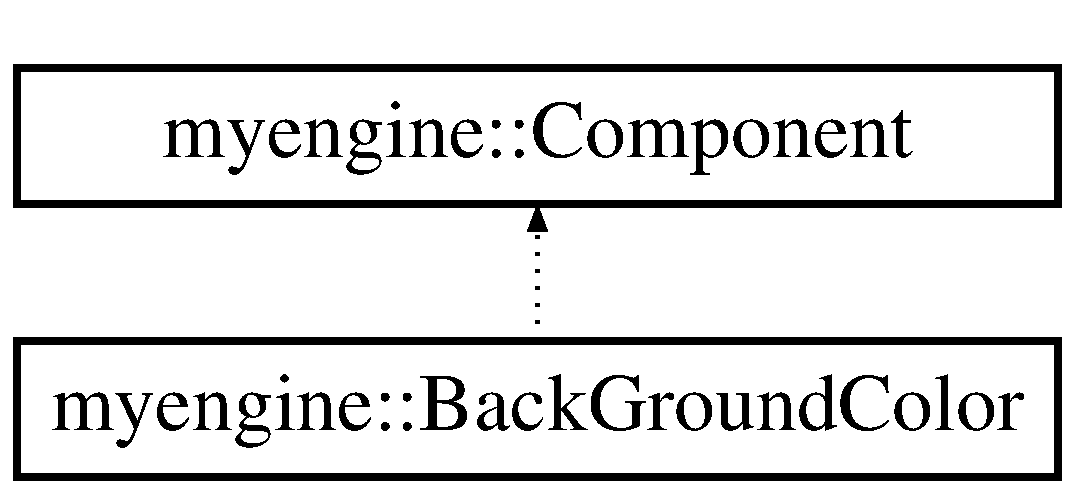
\includegraphics[height=2.000000cm]{classmyengine_1_1_back_ground_color}
\end{center}
\end{figure}


The documentation for this class was generated from the following file\+:\begin{DoxyCompactItemize}
\item 
src/myengine/\hyperlink{_background_color_8h}{Background\+Color.\+h}\end{DoxyCompactItemize}

\hypertarget{classmyengine_1_1_component}{}\section{myengine\+:\+:Component Class Reference}
\label{classmyengine_1_1_component}\index{myengine\+::\+Component@{myengine\+::\+Component}}


{\ttfamily \#include $<$Component.\+h$>$}

Inheritance diagram for myengine\+:\+:Component\+:\begin{figure}[H]
\begin{center}
\leavevmode
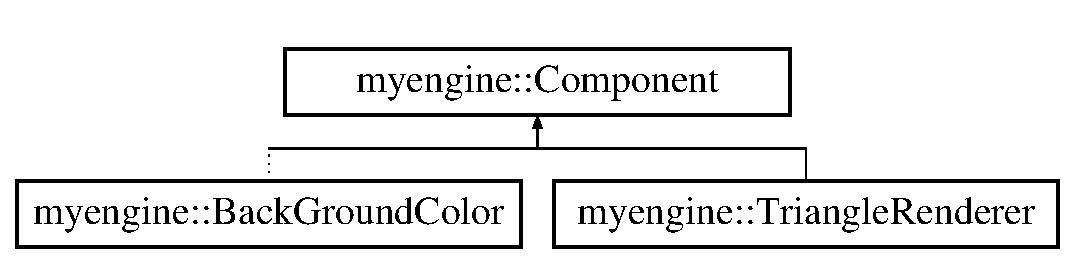
\includegraphics[height=2.000000cm]{classmyengine_1_1_component}
\end{center}
\end{figure}
\subsection*{Public Member Functions}
\begin{DoxyCompactItemize}
\item 
\hyperlink{classmyengine_1_1_component_ae49096ab7e0b46617d28206315bef1a9}{Component} ()
\item 
\hyperlink{classmyengine_1_1_component_ae2938d7961851517b781318a9005ba2c}{$\sim$\+Component} ()
\item 
virtual void \hyperlink{classmyengine_1_1_component_a66aeffd4cb32f438a4fc604e74e50057}{On\+Init} (std\+::weak\+\_\+ptr$<$ \hyperlink{classmyengine_1_1_entity}{Entity} $>$ \+\_\+parent)
\item 
virtual void \hyperlink{classmyengine_1_1_component_ac852700a0c7227ca7229ae8c9ec4aa2d}{On\+Begin} ()
\item 
virtual void \hyperlink{classmyengine_1_1_component_ac84472ba368a622afa0e25c47757291a}{On\+Tick} ()
\item 
virtual void \hyperlink{classmyengine_1_1_component_ade43a7a8f4f8954b45ed05e1a8898eae}{On\+Display} ()
\end{DoxyCompactItemize}
\subsection*{Protected Member Functions}
\begin{DoxyCompactItemize}
\item 
std\+::shared\+\_\+ptr$<$ \hyperlink{classmyengine_1_1_entity}{Entity} $>$ \hyperlink{classmyengine_1_1_component_af409385720cc0c533e8812e8857ba161}{get\+Entity} ()
\item 
std\+::shared\+\_\+ptr$<$ \hyperlink{classmyengine_1_1_core}{Core} $>$ \hyperlink{classmyengine_1_1_component_a2b80c2d91dac8f429f6b6f6305d7c5be}{get\+Core} ()
\item 
std\+::shared\+\_\+ptr$<$ Input $>$ \hyperlink{classmyengine_1_1_component_a3e1451f5c1435ee6d69adf1644075a69}{get\+Input} ()
\item 
std\+::shared\+\_\+ptr$<$ \hyperlink{classmyengine_1_1_environment}{Environment} $>$ \hyperlink{classmyengine_1_1_component_a9b5c293015d5682398462b04cd41ed5a}{get\+Environment} ()
\end{DoxyCompactItemize}


\subsection{Constructor \& Destructor Documentation}
\mbox{\Hypertarget{classmyengine_1_1_component_ae49096ab7e0b46617d28206315bef1a9}\label{classmyengine_1_1_component_ae49096ab7e0b46617d28206315bef1a9}} 
\index{myengine\+::\+Component@{myengine\+::\+Component}!Component@{Component}}
\index{Component@{Component}!myengine\+::\+Component@{myengine\+::\+Component}}
\subsubsection{\texorpdfstring{Component()}{Component()}}
{\footnotesize\ttfamily myengine\+::\+Component\+::\+Component (\begin{DoxyParamCaption}{ }\end{DoxyParamCaption})}

\mbox{\Hypertarget{classmyengine_1_1_component_ae2938d7961851517b781318a9005ba2c}\label{classmyengine_1_1_component_ae2938d7961851517b781318a9005ba2c}} 
\index{myengine\+::\+Component@{myengine\+::\+Component}!````~Component@{$\sim$\+Component}}
\index{````~Component@{$\sim$\+Component}!myengine\+::\+Component@{myengine\+::\+Component}}
\subsubsection{\texorpdfstring{$\sim$\+Component()}{~Component()}}
{\footnotesize\ttfamily myengine\+::\+Component\+::$\sim$\+Component (\begin{DoxyParamCaption}{ }\end{DoxyParamCaption})}



\subsection{Member Function Documentation}
\mbox{\Hypertarget{classmyengine_1_1_component_a2b80c2d91dac8f429f6b6f6305d7c5be}\label{classmyengine_1_1_component_a2b80c2d91dac8f429f6b6f6305d7c5be}} 
\index{myengine\+::\+Component@{myengine\+::\+Component}!get\+Core@{get\+Core}}
\index{get\+Core@{get\+Core}!myengine\+::\+Component@{myengine\+::\+Component}}
\subsubsection{\texorpdfstring{get\+Core()}{getCore()}}
{\footnotesize\ttfamily std\+::shared\+\_\+ptr$<$ \hyperlink{classmyengine_1_1_core}{Core} $>$ myengine\+::\+Component\+::get\+Core (\begin{DoxyParamCaption}{ }\end{DoxyParamCaption})\hspace{0.3cm}{\ttfamily [protected]}}

\mbox{\Hypertarget{classmyengine_1_1_component_af409385720cc0c533e8812e8857ba161}\label{classmyengine_1_1_component_af409385720cc0c533e8812e8857ba161}} 
\index{myengine\+::\+Component@{myengine\+::\+Component}!get\+Entity@{get\+Entity}}
\index{get\+Entity@{get\+Entity}!myengine\+::\+Component@{myengine\+::\+Component}}
\subsubsection{\texorpdfstring{get\+Entity()}{getEntity()}}
{\footnotesize\ttfamily std\+::shared\+\_\+ptr$<$ \hyperlink{classmyengine_1_1_entity}{Entity} $>$ myengine\+::\+Component\+::get\+Entity (\begin{DoxyParamCaption}{ }\end{DoxyParamCaption})\hspace{0.3cm}{\ttfamily [protected]}}

\mbox{\Hypertarget{classmyengine_1_1_component_a9b5c293015d5682398462b04cd41ed5a}\label{classmyengine_1_1_component_a9b5c293015d5682398462b04cd41ed5a}} 
\index{myengine\+::\+Component@{myengine\+::\+Component}!get\+Environment@{get\+Environment}}
\index{get\+Environment@{get\+Environment}!myengine\+::\+Component@{myengine\+::\+Component}}
\subsubsection{\texorpdfstring{get\+Environment()}{getEnvironment()}}
{\footnotesize\ttfamily std\+::shared\+\_\+ptr$<$ \hyperlink{classmyengine_1_1_environment}{Environment} $>$ myengine\+::\+Component\+::get\+Environment (\begin{DoxyParamCaption}{ }\end{DoxyParamCaption})\hspace{0.3cm}{\ttfamily [protected]}}

\mbox{\Hypertarget{classmyengine_1_1_component_a3e1451f5c1435ee6d69adf1644075a69}\label{classmyengine_1_1_component_a3e1451f5c1435ee6d69adf1644075a69}} 
\index{myengine\+::\+Component@{myengine\+::\+Component}!get\+Input@{get\+Input}}
\index{get\+Input@{get\+Input}!myengine\+::\+Component@{myengine\+::\+Component}}
\subsubsection{\texorpdfstring{get\+Input()}{getInput()}}
{\footnotesize\ttfamily std\+::shared\+\_\+ptr$<$ Input $>$ myengine\+::\+Component\+::get\+Input (\begin{DoxyParamCaption}{ }\end{DoxyParamCaption})\hspace{0.3cm}{\ttfamily [protected]}}

\mbox{\Hypertarget{classmyengine_1_1_component_ac852700a0c7227ca7229ae8c9ec4aa2d}\label{classmyengine_1_1_component_ac852700a0c7227ca7229ae8c9ec4aa2d}} 
\index{myengine\+::\+Component@{myengine\+::\+Component}!On\+Begin@{On\+Begin}}
\index{On\+Begin@{On\+Begin}!myengine\+::\+Component@{myengine\+::\+Component}}
\subsubsection{\texorpdfstring{On\+Begin()}{OnBegin()}}
{\footnotesize\ttfamily void myengine\+::\+Component\+::\+On\+Begin (\begin{DoxyParamCaption}{ }\end{DoxyParamCaption})\hspace{0.3cm}{\ttfamily [virtual]}}



Reimplemented in \hyperlink{classmyengine_1_1_triangle_renderer_a74b0a056ed77e78a5061da2da6115bfd}{myengine\+::\+Triangle\+Renderer}.

\mbox{\Hypertarget{classmyengine_1_1_component_ade43a7a8f4f8954b45ed05e1a8898eae}\label{classmyengine_1_1_component_ade43a7a8f4f8954b45ed05e1a8898eae}} 
\index{myengine\+::\+Component@{myengine\+::\+Component}!On\+Display@{On\+Display}}
\index{On\+Display@{On\+Display}!myengine\+::\+Component@{myengine\+::\+Component}}
\subsubsection{\texorpdfstring{On\+Display()}{OnDisplay()}}
{\footnotesize\ttfamily void myengine\+::\+Component\+::\+On\+Display (\begin{DoxyParamCaption}{ }\end{DoxyParamCaption})\hspace{0.3cm}{\ttfamily [virtual]}}



Reimplemented in \hyperlink{classmyengine_1_1_triangle_renderer_a266db93e50781c64232b16fe4f323bad}{myengine\+::\+Triangle\+Renderer}.

\mbox{\Hypertarget{classmyengine_1_1_component_a66aeffd4cb32f438a4fc604e74e50057}\label{classmyengine_1_1_component_a66aeffd4cb32f438a4fc604e74e50057}} 
\index{myengine\+::\+Component@{myengine\+::\+Component}!On\+Init@{On\+Init}}
\index{On\+Init@{On\+Init}!myengine\+::\+Component@{myengine\+::\+Component}}
\subsubsection{\texorpdfstring{On\+Init()}{OnInit()}}
{\footnotesize\ttfamily void myengine\+::\+Component\+::\+On\+Init (\begin{DoxyParamCaption}\item[{std\+::weak\+\_\+ptr$<$ \hyperlink{classmyengine_1_1_entity}{Entity} $>$}]{\+\_\+parent }\end{DoxyParamCaption})\hspace{0.3cm}{\ttfamily [virtual]}}



Reimplemented in \hyperlink{classmyengine_1_1_triangle_renderer_aef2e04f1dd0419df1a60eb0cd95fd86c}{myengine\+::\+Triangle\+Renderer}.

\mbox{\Hypertarget{classmyengine_1_1_component_ac84472ba368a622afa0e25c47757291a}\label{classmyengine_1_1_component_ac84472ba368a622afa0e25c47757291a}} 
\index{myengine\+::\+Component@{myengine\+::\+Component}!On\+Tick@{On\+Tick}}
\index{On\+Tick@{On\+Tick}!myengine\+::\+Component@{myengine\+::\+Component}}
\subsubsection{\texorpdfstring{On\+Tick()}{OnTick()}}
{\footnotesize\ttfamily void myengine\+::\+Component\+::\+On\+Tick (\begin{DoxyParamCaption}{ }\end{DoxyParamCaption})\hspace{0.3cm}{\ttfamily [virtual]}}



Reimplemented in \hyperlink{classmyengine_1_1_triangle_renderer_a6608a9c7954cff50e2575133dd6e5d88}{myengine\+::\+Triangle\+Renderer}.



The documentation for this class was generated from the following files\+:\begin{DoxyCompactItemize}
\item 
src/myengine/\hyperlink{_component_8h}{Component.\+h}\item 
src/myengine/\hyperlink{_component_8cpp}{Component.\+cpp}\end{DoxyCompactItemize}

\hypertarget{classmyengine_1_1_core}{}\section{myengine\+:\+:Core Class Reference}
\label{classmyengine_1_1_core}\index{myengine\+::\+Core@{myengine\+::\+Core}}


{\ttfamily \#include $<$Core.\+h$>$}

Inheritance diagram for myengine\+:\+:Core\+:\begin{figure}[H]
\begin{center}
\leavevmode
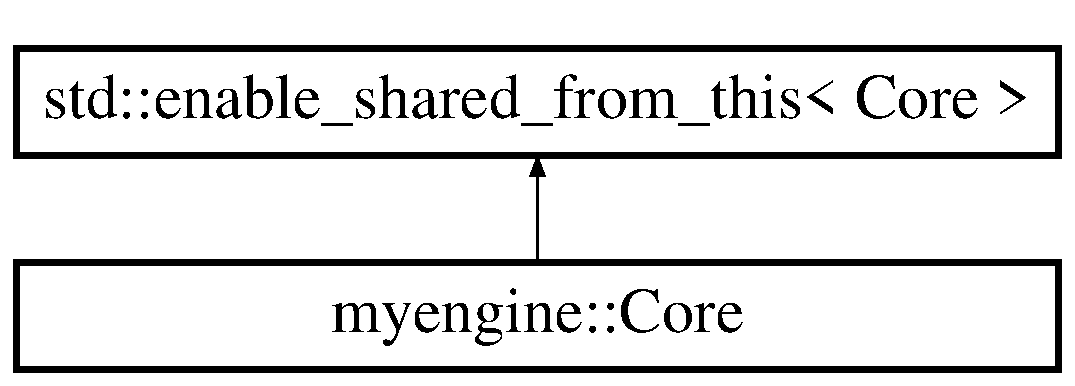
\includegraphics[height=2.000000cm]{classmyengine_1_1_core}
\end{center}
\end{figure}
\subsection*{Public Member Functions}
\begin{DoxyCompactItemize}
\item 
\hyperlink{classmyengine_1_1_core_a51a936e2f539b33caaf91b9b38d5e8da}{Core} ()
\item 
\hyperlink{classmyengine_1_1_core_af8293765bd17b1e0003df3820fa38990}{$\sim$\+Core} ()
\item 
void \hyperlink{classmyengine_1_1_core_aa0e8cb43d17f7294adf039064bc555bc}{Init} ()
\item 
void \hyperlink{classmyengine_1_1_core_ac7ce6b74d6b0228a1b5125ec3373e8b0}{Init} (int \+\_\+width, int \+\_\+height)
\item 
void \hyperlink{classmyengine_1_1_core_a15a52e8674f890144428059b80cf1330}{Start} ()
\item 
void \hyperlink{classmyengine_1_1_core_ab93156cb1b35d422d2827ffe1e431b4a}{Stop} ()
\item 
std\+::shared\+\_\+ptr$<$ \hyperlink{classmyengine_1_1_entity}{Entity} $>$ \hyperlink{classmyengine_1_1_core_abf2eea4d6b0d3788761ea11f34c4981d}{add\+Entity} ()
\item 
std\+::shared\+\_\+ptr$<$ \hyperlink{classmyengine_1_1_environment}{Environment} $>$ \hyperlink{classmyengine_1_1_core_a24c44abbba15cf736ed13c72923863e2}{get\+Environment} ()
\item 
std\+::shared\+\_\+ptr$<$ Input $>$ \hyperlink{classmyengine_1_1_core_ae0824780726297ed16b6ea4d4c009f76}{get\+Input} ()
\item 
std\+::shared\+\_\+ptr$<$ \hyperlink{classmyengine_1_1_resources}{Resources} $>$ \hyperlink{classmyengine_1_1_core_a82f9fc96dd0d9cb9fd29c0aa7cf83c45}{get\+Resources} ()
\item 
void \hyperlink{classmyengine_1_1_core_a250805a435bee8689d7f9bd44c8e7f79}{Set\+Self} (std\+::weak\+\_\+ptr$<$ \hyperlink{classmyengine_1_1_core}{Core} $>$ \+\_\+self\+Ptr)
\end{DoxyCompactItemize}


\subsection{Constructor \& Destructor Documentation}
\mbox{\Hypertarget{classmyengine_1_1_core_a51a936e2f539b33caaf91b9b38d5e8da}\label{classmyengine_1_1_core_a51a936e2f539b33caaf91b9b38d5e8da}} 
\index{myengine\+::\+Core@{myengine\+::\+Core}!Core@{Core}}
\index{Core@{Core}!myengine\+::\+Core@{myengine\+::\+Core}}
\subsubsection{\texorpdfstring{Core()}{Core()}}
{\footnotesize\ttfamily myengine\+::\+Core\+::\+Core (\begin{DoxyParamCaption}{ }\end{DoxyParamCaption})}

\mbox{\Hypertarget{classmyengine_1_1_core_af8293765bd17b1e0003df3820fa38990}\label{classmyengine_1_1_core_af8293765bd17b1e0003df3820fa38990}} 
\index{myengine\+::\+Core@{myengine\+::\+Core}!````~Core@{$\sim$\+Core}}
\index{````~Core@{$\sim$\+Core}!myengine\+::\+Core@{myengine\+::\+Core}}
\subsubsection{\texorpdfstring{$\sim$\+Core()}{~Core()}}
{\footnotesize\ttfamily myengine\+::\+Core\+::$\sim$\+Core (\begin{DoxyParamCaption}{ }\end{DoxyParamCaption})}



\subsection{Member Function Documentation}
\mbox{\Hypertarget{classmyengine_1_1_core_abf2eea4d6b0d3788761ea11f34c4981d}\label{classmyengine_1_1_core_abf2eea4d6b0d3788761ea11f34c4981d}} 
\index{myengine\+::\+Core@{myengine\+::\+Core}!add\+Entity@{add\+Entity}}
\index{add\+Entity@{add\+Entity}!myengine\+::\+Core@{myengine\+::\+Core}}
\subsubsection{\texorpdfstring{add\+Entity()}{addEntity()}}
{\footnotesize\ttfamily std\+::shared\+\_\+ptr$<$ \hyperlink{classmyengine_1_1_entity}{Entity} $>$ myengine\+::\+Core\+::add\+Entity (\begin{DoxyParamCaption}{ }\end{DoxyParamCaption})}

\mbox{\Hypertarget{classmyengine_1_1_core_a24c44abbba15cf736ed13c72923863e2}\label{classmyengine_1_1_core_a24c44abbba15cf736ed13c72923863e2}} 
\index{myengine\+::\+Core@{myengine\+::\+Core}!get\+Environment@{get\+Environment}}
\index{get\+Environment@{get\+Environment}!myengine\+::\+Core@{myengine\+::\+Core}}
\subsubsection{\texorpdfstring{get\+Environment()}{getEnvironment()}}
{\footnotesize\ttfamily std\+::shared\+\_\+ptr$<$ \hyperlink{classmyengine_1_1_environment}{Environment} $>$ myengine\+::\+Core\+::get\+Environment (\begin{DoxyParamCaption}{ }\end{DoxyParamCaption})}

\mbox{\Hypertarget{classmyengine_1_1_core_ae0824780726297ed16b6ea4d4c009f76}\label{classmyengine_1_1_core_ae0824780726297ed16b6ea4d4c009f76}} 
\index{myengine\+::\+Core@{myengine\+::\+Core}!get\+Input@{get\+Input}}
\index{get\+Input@{get\+Input}!myengine\+::\+Core@{myengine\+::\+Core}}
\subsubsection{\texorpdfstring{get\+Input()}{getInput()}}
{\footnotesize\ttfamily std\+::shared\+\_\+ptr$<$ Input $>$ myengine\+::\+Core\+::get\+Input (\begin{DoxyParamCaption}{ }\end{DoxyParamCaption})}

\mbox{\Hypertarget{classmyengine_1_1_core_a82f9fc96dd0d9cb9fd29c0aa7cf83c45}\label{classmyengine_1_1_core_a82f9fc96dd0d9cb9fd29c0aa7cf83c45}} 
\index{myengine\+::\+Core@{myengine\+::\+Core}!get\+Resources@{get\+Resources}}
\index{get\+Resources@{get\+Resources}!myengine\+::\+Core@{myengine\+::\+Core}}
\subsubsection{\texorpdfstring{get\+Resources()}{getResources()}}
{\footnotesize\ttfamily std\+::shared\+\_\+ptr$<$ \hyperlink{classmyengine_1_1_resources}{Resources} $>$ myengine\+::\+Core\+::get\+Resources (\begin{DoxyParamCaption}{ }\end{DoxyParamCaption})}

\mbox{\Hypertarget{classmyengine_1_1_core_aa0e8cb43d17f7294adf039064bc555bc}\label{classmyengine_1_1_core_aa0e8cb43d17f7294adf039064bc555bc}} 
\index{myengine\+::\+Core@{myengine\+::\+Core}!Init@{Init}}
\index{Init@{Init}!myengine\+::\+Core@{myengine\+::\+Core}}
\subsubsection{\texorpdfstring{Init()}{Init()}\hspace{0.1cm}{\footnotesize\ttfamily [1/2]}}
{\footnotesize\ttfamily void myengine\+::\+Core\+::\+Init (\begin{DoxyParamCaption}{ }\end{DoxyParamCaption})}

\mbox{\Hypertarget{classmyengine_1_1_core_ac7ce6b74d6b0228a1b5125ec3373e8b0}\label{classmyengine_1_1_core_ac7ce6b74d6b0228a1b5125ec3373e8b0}} 
\index{myengine\+::\+Core@{myengine\+::\+Core}!Init@{Init}}
\index{Init@{Init}!myengine\+::\+Core@{myengine\+::\+Core}}
\subsubsection{\texorpdfstring{Init()}{Init()}\hspace{0.1cm}{\footnotesize\ttfamily [2/2]}}
{\footnotesize\ttfamily void myengine\+::\+Core\+::\+Init (\begin{DoxyParamCaption}\item[{int}]{\+\_\+width,  }\item[{int}]{\+\_\+height }\end{DoxyParamCaption})}

\mbox{\Hypertarget{classmyengine_1_1_core_a250805a435bee8689d7f9bd44c8e7f79}\label{classmyengine_1_1_core_a250805a435bee8689d7f9bd44c8e7f79}} 
\index{myengine\+::\+Core@{myengine\+::\+Core}!Set\+Self@{Set\+Self}}
\index{Set\+Self@{Set\+Self}!myengine\+::\+Core@{myengine\+::\+Core}}
\subsubsection{\texorpdfstring{Set\+Self()}{SetSelf()}}
{\footnotesize\ttfamily void myengine\+::\+Core\+::\+Set\+Self (\begin{DoxyParamCaption}\item[{std\+::weak\+\_\+ptr$<$ \hyperlink{classmyengine_1_1_core}{Core} $>$}]{\+\_\+self\+Ptr }\end{DoxyParamCaption})}

\mbox{\Hypertarget{classmyengine_1_1_core_a15a52e8674f890144428059b80cf1330}\label{classmyengine_1_1_core_a15a52e8674f890144428059b80cf1330}} 
\index{myengine\+::\+Core@{myengine\+::\+Core}!Start@{Start}}
\index{Start@{Start}!myengine\+::\+Core@{myengine\+::\+Core}}
\subsubsection{\texorpdfstring{Start()}{Start()}}
{\footnotesize\ttfamily void myengine\+::\+Core\+::\+Start (\begin{DoxyParamCaption}{ }\end{DoxyParamCaption})}

\mbox{\Hypertarget{classmyengine_1_1_core_ab93156cb1b35d422d2827ffe1e431b4a}\label{classmyengine_1_1_core_ab93156cb1b35d422d2827ffe1e431b4a}} 
\index{myengine\+::\+Core@{myengine\+::\+Core}!Stop@{Stop}}
\index{Stop@{Stop}!myengine\+::\+Core@{myengine\+::\+Core}}
\subsubsection{\texorpdfstring{Stop()}{Stop()}}
{\footnotesize\ttfamily void myengine\+::\+Core\+::\+Stop (\begin{DoxyParamCaption}{ }\end{DoxyParamCaption})}



The documentation for this class was generated from the following files\+:\begin{DoxyCompactItemize}
\item 
src/myengine/\hyperlink{_core_8h}{Core.\+h}\item 
src/myengine/\hyperlink{_core_8cpp}{Core.\+cpp}\end{DoxyCompactItemize}

\hypertarget{classmyengine_1_1_entity}{}\section{myengine\+:\+:Entity Class Reference}
\label{classmyengine_1_1_entity}\index{myengine\+::\+Entity@{myengine\+::\+Entity}}


{\ttfamily \#include $<$Entity.\+h$>$}

Inheritance diagram for myengine\+:\+:Entity\+:\begin{figure}[H]
\begin{center}
\leavevmode
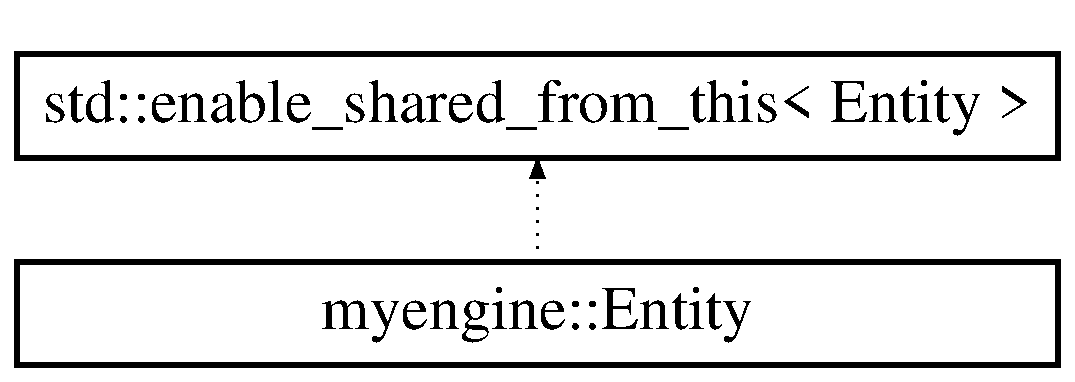
\includegraphics[height=2.000000cm]{classmyengine_1_1_entity}
\end{center}
\end{figure}
\subsection*{Public Member Functions}
\begin{DoxyCompactItemize}
\item 
\hyperlink{classmyengine_1_1_entity_a5d604268b8ba4244f61bb94f94cd733e}{Entity} ()
\item 
\hyperlink{classmyengine_1_1_entity_a1f09697ca205ce1322e33b8e30c6fd98}{$\sim$\+Entity} ()
\item 
void \hyperlink{classmyengine_1_1_entity_a8b69d2ad88cb674d36b14251d8795d9c}{init} (std\+::weak\+\_\+ptr$<$ \hyperlink{classmyengine_1_1_core}{Core} $>$ \+\_\+core\+Ptr)
\item 
std\+::shared\+\_\+ptr$<$ \hyperlink{classmyengine_1_1_core}{Core} $>$ \hyperlink{classmyengine_1_1_entity_a1d39705dcf1bb5022b03d52f7622da31}{get\+Core} ()
\item 
void \hyperlink{classmyengine_1_1_entity_ab0a125079867c099760260086386f4c2}{tick} ()
\item 
void \hyperlink{classmyengine_1_1_entity_a04394bae3f2ce6b6ee0cd2e2a0d62898}{set\+Self} (std\+::weak\+\_\+ptr$<$ \hyperlink{classmyengine_1_1_entity}{Entity} $>$ \+\_\+self\+Ptr)
\item 
{\footnotesize template$<$typename T $>$ }\\std\+::shared\+\_\+ptr$<$ T $>$ \hyperlink{classmyengine_1_1_entity_a2c69500893f016340c50603e9fa1910c}{add\+Component} ()
\item 
{\footnotesize template$<$typename T , typename A $>$ }\\std\+::shared\+\_\+ptr$<$ T $>$ \hyperlink{classmyengine_1_1_entity_acb1f6835d2682b472c15ea3f9549cf06}{add\+Component} (A \+\_\+a)
\item 
{\footnotesize template$<$typename T , typename A , typename B $>$ }\\std\+::shared\+\_\+ptr$<$ T $>$ \hyperlink{classmyengine_1_1_entity_a699b9337feb98eb1710124e2342f6b08}{add\+Component} (A \+\_\+a, B \+\_\+b)
\item 
{\footnotesize template$<$typename T , typename A , typename B , typename C $>$ }\\std\+::shared\+\_\+ptr$<$ T $>$ \hyperlink{classmyengine_1_1_entity_a0565fdbc952c09573366f081f0a7cb39}{add\+Component} (A \+\_\+a, B \+\_\+b, C \+\_\+c)
\item 
{\footnotesize template$<$typename T , typename A , typename B , typename C , typename D $>$ }\\std\+::shared\+\_\+ptr$<$ T $>$ \hyperlink{classmyengine_1_1_entity_ad2a7f70c6260d632660be1b87940d34f}{add\+Component} (A \+\_\+a, B \+\_\+b, C \+\_\+c, D \+\_\+d)
\item 
{\footnotesize template$<$typename T $>$ }\\std\+::shared\+\_\+ptr$<$ T $>$ \hyperlink{classmyengine_1_1_entity_a4c9766055bdda5a8c398417c66e085b9}{get\+Component} ()
\end{DoxyCompactItemize}


\subsection{Constructor \& Destructor Documentation}
\mbox{\Hypertarget{classmyengine_1_1_entity_a5d604268b8ba4244f61bb94f94cd733e}\label{classmyengine_1_1_entity_a5d604268b8ba4244f61bb94f94cd733e}} 
\index{myengine\+::\+Entity@{myengine\+::\+Entity}!Entity@{Entity}}
\index{Entity@{Entity}!myengine\+::\+Entity@{myengine\+::\+Entity}}
\subsubsection{\texorpdfstring{Entity()}{Entity()}}
{\footnotesize\ttfamily myengine\+::\+Entity\+::\+Entity (\begin{DoxyParamCaption}{ }\end{DoxyParamCaption})}

\mbox{\Hypertarget{classmyengine_1_1_entity_a1f09697ca205ce1322e33b8e30c6fd98}\label{classmyengine_1_1_entity_a1f09697ca205ce1322e33b8e30c6fd98}} 
\index{myengine\+::\+Entity@{myengine\+::\+Entity}!````~Entity@{$\sim$\+Entity}}
\index{````~Entity@{$\sim$\+Entity}!myengine\+::\+Entity@{myengine\+::\+Entity}}
\subsubsection{\texorpdfstring{$\sim$\+Entity()}{~Entity()}}
{\footnotesize\ttfamily myengine\+::\+Entity\+::$\sim$\+Entity (\begin{DoxyParamCaption}{ }\end{DoxyParamCaption})}



\subsection{Member Function Documentation}
\mbox{\Hypertarget{classmyengine_1_1_entity_a2c69500893f016340c50603e9fa1910c}\label{classmyengine_1_1_entity_a2c69500893f016340c50603e9fa1910c}} 
\index{myengine\+::\+Entity@{myengine\+::\+Entity}!add\+Component@{add\+Component}}
\index{add\+Component@{add\+Component}!myengine\+::\+Entity@{myengine\+::\+Entity}}
\subsubsection{\texorpdfstring{add\+Component()}{addComponent()}\hspace{0.1cm}{\footnotesize\ttfamily [1/5]}}
{\footnotesize\ttfamily template$<$typename T $>$ \\
std\+::shared\+\_\+ptr$<$T$>$ myengine\+::\+Entity\+::add\+Component (\begin{DoxyParamCaption}{ }\end{DoxyParamCaption})\hspace{0.3cm}{\ttfamily [inline]}}

\mbox{\Hypertarget{classmyengine_1_1_entity_acb1f6835d2682b472c15ea3f9549cf06}\label{classmyengine_1_1_entity_acb1f6835d2682b472c15ea3f9549cf06}} 
\index{myengine\+::\+Entity@{myengine\+::\+Entity}!add\+Component@{add\+Component}}
\index{add\+Component@{add\+Component}!myengine\+::\+Entity@{myengine\+::\+Entity}}
\subsubsection{\texorpdfstring{add\+Component()}{addComponent()}\hspace{0.1cm}{\footnotesize\ttfamily [2/5]}}
{\footnotesize\ttfamily template$<$typename T , typename A $>$ \\
std\+::shared\+\_\+ptr$<$T$>$ myengine\+::\+Entity\+::add\+Component (\begin{DoxyParamCaption}\item[{A}]{\+\_\+a }\end{DoxyParamCaption})\hspace{0.3cm}{\ttfamily [inline]}}

\mbox{\Hypertarget{classmyengine_1_1_entity_a699b9337feb98eb1710124e2342f6b08}\label{classmyengine_1_1_entity_a699b9337feb98eb1710124e2342f6b08}} 
\index{myengine\+::\+Entity@{myengine\+::\+Entity}!add\+Component@{add\+Component}}
\index{add\+Component@{add\+Component}!myengine\+::\+Entity@{myengine\+::\+Entity}}
\subsubsection{\texorpdfstring{add\+Component()}{addComponent()}\hspace{0.1cm}{\footnotesize\ttfamily [3/5]}}
{\footnotesize\ttfamily template$<$typename T , typename A , typename B $>$ \\
std\+::shared\+\_\+ptr$<$T$>$ myengine\+::\+Entity\+::add\+Component (\begin{DoxyParamCaption}\item[{A}]{\+\_\+a,  }\item[{B}]{\+\_\+b }\end{DoxyParamCaption})\hspace{0.3cm}{\ttfamily [inline]}}

\mbox{\Hypertarget{classmyengine_1_1_entity_a0565fdbc952c09573366f081f0a7cb39}\label{classmyengine_1_1_entity_a0565fdbc952c09573366f081f0a7cb39}} 
\index{myengine\+::\+Entity@{myengine\+::\+Entity}!add\+Component@{add\+Component}}
\index{add\+Component@{add\+Component}!myengine\+::\+Entity@{myengine\+::\+Entity}}
\subsubsection{\texorpdfstring{add\+Component()}{addComponent()}\hspace{0.1cm}{\footnotesize\ttfamily [4/5]}}
{\footnotesize\ttfamily template$<$typename T , typename A , typename B , typename C $>$ \\
std\+::shared\+\_\+ptr$<$T$>$ myengine\+::\+Entity\+::add\+Component (\begin{DoxyParamCaption}\item[{A}]{\+\_\+a,  }\item[{B}]{\+\_\+b,  }\item[{C}]{\+\_\+c }\end{DoxyParamCaption})\hspace{0.3cm}{\ttfamily [inline]}}

\mbox{\Hypertarget{classmyengine_1_1_entity_ad2a7f70c6260d632660be1b87940d34f}\label{classmyengine_1_1_entity_ad2a7f70c6260d632660be1b87940d34f}} 
\index{myengine\+::\+Entity@{myengine\+::\+Entity}!add\+Component@{add\+Component}}
\index{add\+Component@{add\+Component}!myengine\+::\+Entity@{myengine\+::\+Entity}}
\subsubsection{\texorpdfstring{add\+Component()}{addComponent()}\hspace{0.1cm}{\footnotesize\ttfamily [5/5]}}
{\footnotesize\ttfamily template$<$typename T , typename A , typename B , typename C , typename D $>$ \\
std\+::shared\+\_\+ptr$<$T$>$ myengine\+::\+Entity\+::add\+Component (\begin{DoxyParamCaption}\item[{A}]{\+\_\+a,  }\item[{B}]{\+\_\+b,  }\item[{C}]{\+\_\+c,  }\item[{D}]{\+\_\+d }\end{DoxyParamCaption})\hspace{0.3cm}{\ttfamily [inline]}}

\mbox{\Hypertarget{classmyengine_1_1_entity_a4c9766055bdda5a8c398417c66e085b9}\label{classmyengine_1_1_entity_a4c9766055bdda5a8c398417c66e085b9}} 
\index{myengine\+::\+Entity@{myengine\+::\+Entity}!get\+Component@{get\+Component}}
\index{get\+Component@{get\+Component}!myengine\+::\+Entity@{myengine\+::\+Entity}}
\subsubsection{\texorpdfstring{get\+Component()}{getComponent()}}
{\footnotesize\ttfamily template$<$typename T $>$ \\
std\+::shared\+\_\+ptr$<$T$>$ myengine\+::\+Entity\+::get\+Component (\begin{DoxyParamCaption}{ }\end{DoxyParamCaption})\hspace{0.3cm}{\ttfamily [inline]}}

\mbox{\Hypertarget{classmyengine_1_1_entity_a1d39705dcf1bb5022b03d52f7622da31}\label{classmyengine_1_1_entity_a1d39705dcf1bb5022b03d52f7622da31}} 
\index{myengine\+::\+Entity@{myengine\+::\+Entity}!get\+Core@{get\+Core}}
\index{get\+Core@{get\+Core}!myengine\+::\+Entity@{myengine\+::\+Entity}}
\subsubsection{\texorpdfstring{get\+Core()}{getCore()}}
{\footnotesize\ttfamily std\+::shared\+\_\+ptr$<$ \hyperlink{classmyengine_1_1_core}{Core} $>$ myengine\+::\+Entity\+::get\+Core (\begin{DoxyParamCaption}{ }\end{DoxyParamCaption})}

\mbox{\Hypertarget{classmyengine_1_1_entity_a8b69d2ad88cb674d36b14251d8795d9c}\label{classmyengine_1_1_entity_a8b69d2ad88cb674d36b14251d8795d9c}} 
\index{myengine\+::\+Entity@{myengine\+::\+Entity}!init@{init}}
\index{init@{init}!myengine\+::\+Entity@{myengine\+::\+Entity}}
\subsubsection{\texorpdfstring{init()}{init()}}
{\footnotesize\ttfamily void myengine\+::\+Entity\+::init (\begin{DoxyParamCaption}\item[{std\+::weak\+\_\+ptr$<$ \hyperlink{classmyengine_1_1_core}{Core} $>$}]{\+\_\+core\+Ptr }\end{DoxyParamCaption})}

\mbox{\Hypertarget{classmyengine_1_1_entity_a04394bae3f2ce6b6ee0cd2e2a0d62898}\label{classmyengine_1_1_entity_a04394bae3f2ce6b6ee0cd2e2a0d62898}} 
\index{myengine\+::\+Entity@{myengine\+::\+Entity}!set\+Self@{set\+Self}}
\index{set\+Self@{set\+Self}!myengine\+::\+Entity@{myengine\+::\+Entity}}
\subsubsection{\texorpdfstring{set\+Self()}{setSelf()}}
{\footnotesize\ttfamily void myengine\+::\+Entity\+::set\+Self (\begin{DoxyParamCaption}\item[{std\+::weak\+\_\+ptr$<$ \hyperlink{classmyengine_1_1_entity}{Entity} $>$}]{\+\_\+self\+Ptr }\end{DoxyParamCaption})}

\mbox{\Hypertarget{classmyengine_1_1_entity_ab0a125079867c099760260086386f4c2}\label{classmyengine_1_1_entity_ab0a125079867c099760260086386f4c2}} 
\index{myengine\+::\+Entity@{myengine\+::\+Entity}!tick@{tick}}
\index{tick@{tick}!myengine\+::\+Entity@{myengine\+::\+Entity}}
\subsubsection{\texorpdfstring{tick()}{tick()}}
{\footnotesize\ttfamily void myengine\+::\+Entity\+::tick (\begin{DoxyParamCaption}{ }\end{DoxyParamCaption})}



The documentation for this class was generated from the following files\+:\begin{DoxyCompactItemize}
\item 
src/myengine/\hyperlink{_entity_8h}{Entity.\+h}\item 
src/myengine/\hyperlink{_entity_8cpp}{Entity.\+cpp}\end{DoxyCompactItemize}

\hypertarget{classmyengine_1_1_environment}{}\section{myengine\+:\+:Environment Class Reference}
\label{classmyengine_1_1_environment}\index{myengine\+::\+Environment@{myengine\+::\+Environment}}


{\ttfamily \#include $<$Environment.\+h$>$}

\subsection*{Public Member Functions}
\begin{DoxyCompactItemize}
\item 
\hyperlink{classmyengine_1_1_environment_a3b0875e176697100bcc7e56671e9a3b1}{Environment} ()
\item 
\hyperlink{classmyengine_1_1_environment_a9e1bcf2cb77d6b5729e4d66006c88ce7}{$\sim$\+Environment} ()
\item 
float \hyperlink{classmyengine_1_1_environment_aa1f6d8ffc9d9cce24c9fd6b86445ccbc}{get\+Delta\+Time} ()
\item 
void \hyperlink{classmyengine_1_1_environment_a899c1088832b702e5c4e7d309a68e8fb}{tick} ()
\end{DoxyCompactItemize}


\subsection{Constructor \& Destructor Documentation}
\mbox{\Hypertarget{classmyengine_1_1_environment_a3b0875e176697100bcc7e56671e9a3b1}\label{classmyengine_1_1_environment_a3b0875e176697100bcc7e56671e9a3b1}} 
\index{myengine\+::\+Environment@{myengine\+::\+Environment}!Environment@{Environment}}
\index{Environment@{Environment}!myengine\+::\+Environment@{myengine\+::\+Environment}}
\subsubsection{\texorpdfstring{Environment()}{Environment()}}
{\footnotesize\ttfamily myengine\+::\+Environment\+::\+Environment (\begin{DoxyParamCaption}{ }\end{DoxyParamCaption})}

\mbox{\Hypertarget{classmyengine_1_1_environment_a9e1bcf2cb77d6b5729e4d66006c88ce7}\label{classmyengine_1_1_environment_a9e1bcf2cb77d6b5729e4d66006c88ce7}} 
\index{myengine\+::\+Environment@{myengine\+::\+Environment}!````~Environment@{$\sim$\+Environment}}
\index{````~Environment@{$\sim$\+Environment}!myengine\+::\+Environment@{myengine\+::\+Environment}}
\subsubsection{\texorpdfstring{$\sim$\+Environment()}{~Environment()}}
{\footnotesize\ttfamily myengine\+::\+Environment\+::$\sim$\+Environment (\begin{DoxyParamCaption}{ }\end{DoxyParamCaption})}



\subsection{Member Function Documentation}
\mbox{\Hypertarget{classmyengine_1_1_environment_aa1f6d8ffc9d9cce24c9fd6b86445ccbc}\label{classmyengine_1_1_environment_aa1f6d8ffc9d9cce24c9fd6b86445ccbc}} 
\index{myengine\+::\+Environment@{myengine\+::\+Environment}!get\+Delta\+Time@{get\+Delta\+Time}}
\index{get\+Delta\+Time@{get\+Delta\+Time}!myengine\+::\+Environment@{myengine\+::\+Environment}}
\subsubsection{\texorpdfstring{get\+Delta\+Time()}{getDeltaTime()}}
{\footnotesize\ttfamily float myengine\+::\+Environment\+::get\+Delta\+Time (\begin{DoxyParamCaption}{ }\end{DoxyParamCaption})}

\mbox{\Hypertarget{classmyengine_1_1_environment_a899c1088832b702e5c4e7d309a68e8fb}\label{classmyengine_1_1_environment_a899c1088832b702e5c4e7d309a68e8fb}} 
\index{myengine\+::\+Environment@{myengine\+::\+Environment}!tick@{tick}}
\index{tick@{tick}!myengine\+::\+Environment@{myengine\+::\+Environment}}
\subsubsection{\texorpdfstring{tick()}{tick()}}
{\footnotesize\ttfamily void myengine\+::\+Environment\+::tick (\begin{DoxyParamCaption}{ }\end{DoxyParamCaption})}



The documentation for this class was generated from the following files\+:\begin{DoxyCompactItemize}
\item 
src/myengine/\hyperlink{_environment_8h}{Environment.\+h}\item 
src/myengine/\hyperlink{_environment_8cpp}{Environment.\+cpp}\end{DoxyCompactItemize}

\hypertarget{classmyengine_1_1_resource}{}\section{myengine\+:\+:Resource Class Reference}
\label{classmyengine_1_1_resource}\index{myengine\+::\+Resource@{myengine\+::\+Resource}}


{\ttfamily \#include $<$Resource.\+h$>$}

Inheritance diagram for myengine\+:\+:Resource\+:\begin{figure}[H]
\begin{center}
\leavevmode
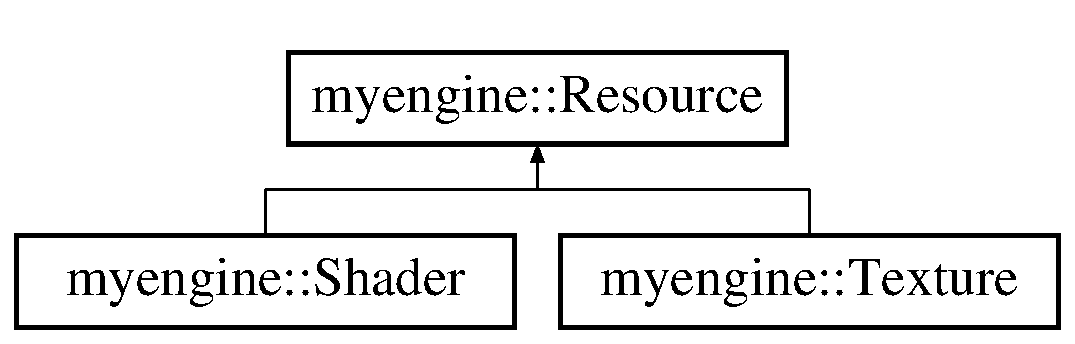
\includegraphics[height=2.000000cm]{classmyengine_1_1_resource}
\end{center}
\end{figure}
\subsection*{Public Member Functions}
\begin{DoxyCompactItemize}
\item 
\hyperlink{classmyengine_1_1_resource_ab6fa75b1f7c8c76714987e99560feb1f}{Resource} ()
\item 
\hyperlink{classmyengine_1_1_resource_a9201d21cadaff21f148143b508e8d667}{Resource} (std\+::string \+\_\+path\+Str)
\item 
\hyperlink{classmyengine_1_1_resource_a450384125daf3876d16ee6f655dce578}{$\sim$\+Resource} ()
\end{DoxyCompactItemize}
\subsection*{Protected Attributes}
\begin{DoxyCompactItemize}
\item 
std\+::string \hyperlink{classmyengine_1_1_resource_af7057ebf099efbd80751c64d25c2c83d}{\+\_\+path}
\end{DoxyCompactItemize}


\subsection{Constructor \& Destructor Documentation}
\mbox{\Hypertarget{classmyengine_1_1_resource_ab6fa75b1f7c8c76714987e99560feb1f}\label{classmyengine_1_1_resource_ab6fa75b1f7c8c76714987e99560feb1f}} 
\index{myengine\+::\+Resource@{myengine\+::\+Resource}!Resource@{Resource}}
\index{Resource@{Resource}!myengine\+::\+Resource@{myengine\+::\+Resource}}
\subsubsection{\texorpdfstring{Resource()}{Resource()}\hspace{0.1cm}{\footnotesize\ttfamily [1/2]}}
{\footnotesize\ttfamily myengine\+::\+Resource\+::\+Resource (\begin{DoxyParamCaption}{ }\end{DoxyParamCaption})}

\mbox{\Hypertarget{classmyengine_1_1_resource_a9201d21cadaff21f148143b508e8d667}\label{classmyengine_1_1_resource_a9201d21cadaff21f148143b508e8d667}} 
\index{myengine\+::\+Resource@{myengine\+::\+Resource}!Resource@{Resource}}
\index{Resource@{Resource}!myengine\+::\+Resource@{myengine\+::\+Resource}}
\subsubsection{\texorpdfstring{Resource()}{Resource()}\hspace{0.1cm}{\footnotesize\ttfamily [2/2]}}
{\footnotesize\ttfamily myengine\+::\+Resource\+::\+Resource (\begin{DoxyParamCaption}\item[{std\+::string}]{\+\_\+path\+Str }\end{DoxyParamCaption})}

\mbox{\Hypertarget{classmyengine_1_1_resource_a450384125daf3876d16ee6f655dce578}\label{classmyengine_1_1_resource_a450384125daf3876d16ee6f655dce578}} 
\index{myengine\+::\+Resource@{myengine\+::\+Resource}!````~Resource@{$\sim$\+Resource}}
\index{````~Resource@{$\sim$\+Resource}!myengine\+::\+Resource@{myengine\+::\+Resource}}
\subsubsection{\texorpdfstring{$\sim$\+Resource()}{~Resource()}}
{\footnotesize\ttfamily myengine\+::\+Resource\+::$\sim$\+Resource (\begin{DoxyParamCaption}{ }\end{DoxyParamCaption})}



\subsection{Member Data Documentation}
\mbox{\Hypertarget{classmyengine_1_1_resource_af7057ebf099efbd80751c64d25c2c83d}\label{classmyengine_1_1_resource_af7057ebf099efbd80751c64d25c2c83d}} 
\index{myengine\+::\+Resource@{myengine\+::\+Resource}!\+\_\+path@{\+\_\+path}}
\index{\+\_\+path@{\+\_\+path}!myengine\+::\+Resource@{myengine\+::\+Resource}}
\subsubsection{\texorpdfstring{\+\_\+path}{\_path}}
{\footnotesize\ttfamily std\+::string myengine\+::\+Resource\+::\+\_\+path\hspace{0.3cm}{\ttfamily [protected]}}



The documentation for this class was generated from the following files\+:\begin{DoxyCompactItemize}
\item 
src/myengine/\hyperlink{_resource_8h}{Resource.\+h}\item 
src/myengine/\hyperlink{_resource_8cpp}{Resource.\+cpp}\end{DoxyCompactItemize}

\hypertarget{classmyengine_1_1_resources}{}\section{myengine\+:\+:Resources Class Reference}
\label{classmyengine_1_1_resources}\index{myengine\+::\+Resources@{myengine\+::\+Resources}}


{\ttfamily \#include $<$Resources.\+h$>$}

\subsection*{Public Member Functions}
\begin{DoxyCompactItemize}
\item 
\hyperlink{classmyengine_1_1_resources_a510c0c94b6b153ab2513f13bc114a7b1}{Resources} ()
\item 
\hyperlink{classmyengine_1_1_resources_a70ec392cd9f38bb1752f868c00a755c6}{$\sim$\+Resources} ()
\item 
void \hyperlink{classmyengine_1_1_resources_aec0d326b9f0e38e6f1aab9c6ecbaf733}{Add\+Created\+Resource} (std\+::shared\+\_\+ptr$<$ \hyperlink{classmyengine_1_1_resource}{Resource} $>$ \+\_\+resource)
\end{DoxyCompactItemize}


\subsection{Constructor \& Destructor Documentation}
\mbox{\Hypertarget{classmyengine_1_1_resources_a510c0c94b6b153ab2513f13bc114a7b1}\label{classmyengine_1_1_resources_a510c0c94b6b153ab2513f13bc114a7b1}} 
\index{myengine\+::\+Resources@{myengine\+::\+Resources}!Resources@{Resources}}
\index{Resources@{Resources}!myengine\+::\+Resources@{myengine\+::\+Resources}}
\subsubsection{\texorpdfstring{Resources()}{Resources()}}
{\footnotesize\ttfamily myengine\+::\+Resources\+::\+Resources (\begin{DoxyParamCaption}{ }\end{DoxyParamCaption})}

\mbox{\Hypertarget{classmyengine_1_1_resources_a70ec392cd9f38bb1752f868c00a755c6}\label{classmyengine_1_1_resources_a70ec392cd9f38bb1752f868c00a755c6}} 
\index{myengine\+::\+Resources@{myengine\+::\+Resources}!````~Resources@{$\sim$\+Resources}}
\index{````~Resources@{$\sim$\+Resources}!myengine\+::\+Resources@{myengine\+::\+Resources}}
\subsubsection{\texorpdfstring{$\sim$\+Resources()}{~Resources()}}
{\footnotesize\ttfamily myengine\+::\+Resources\+::$\sim$\+Resources (\begin{DoxyParamCaption}{ }\end{DoxyParamCaption})}



\subsection{Member Function Documentation}
\mbox{\Hypertarget{classmyengine_1_1_resources_aec0d326b9f0e38e6f1aab9c6ecbaf733}\label{classmyengine_1_1_resources_aec0d326b9f0e38e6f1aab9c6ecbaf733}} 
\index{myengine\+::\+Resources@{myengine\+::\+Resources}!Add\+Created\+Resource@{Add\+Created\+Resource}}
\index{Add\+Created\+Resource@{Add\+Created\+Resource}!myengine\+::\+Resources@{myengine\+::\+Resources}}
\subsubsection{\texorpdfstring{Add\+Created\+Resource()}{AddCreatedResource()}}
{\footnotesize\ttfamily void myengine\+::\+Resources\+::\+Add\+Created\+Resource (\begin{DoxyParamCaption}\item[{std\+::shared\+\_\+ptr$<$ \hyperlink{classmyengine_1_1_resource}{Resource} $>$}]{\+\_\+resource }\end{DoxyParamCaption})}



The documentation for this class was generated from the following files\+:\begin{DoxyCompactItemize}
\item 
src/myengine/\hyperlink{_resources_8h}{Resources.\+h}\item 
src/myengine/\hyperlink{_resources_8cpp}{Resources.\+cpp}\end{DoxyCompactItemize}

\hypertarget{classmyengine_1_1_shader}{}\section{myengine\+:\+:Shader Class Reference}
\label{classmyengine_1_1_shader}\index{myengine\+::\+Shader@{myengine\+::\+Shader}}


{\ttfamily \#include $<$Shader.\+h$>$}

Inheritance diagram for myengine\+:\+:Shader\+:\begin{figure}[H]
\begin{center}
\leavevmode
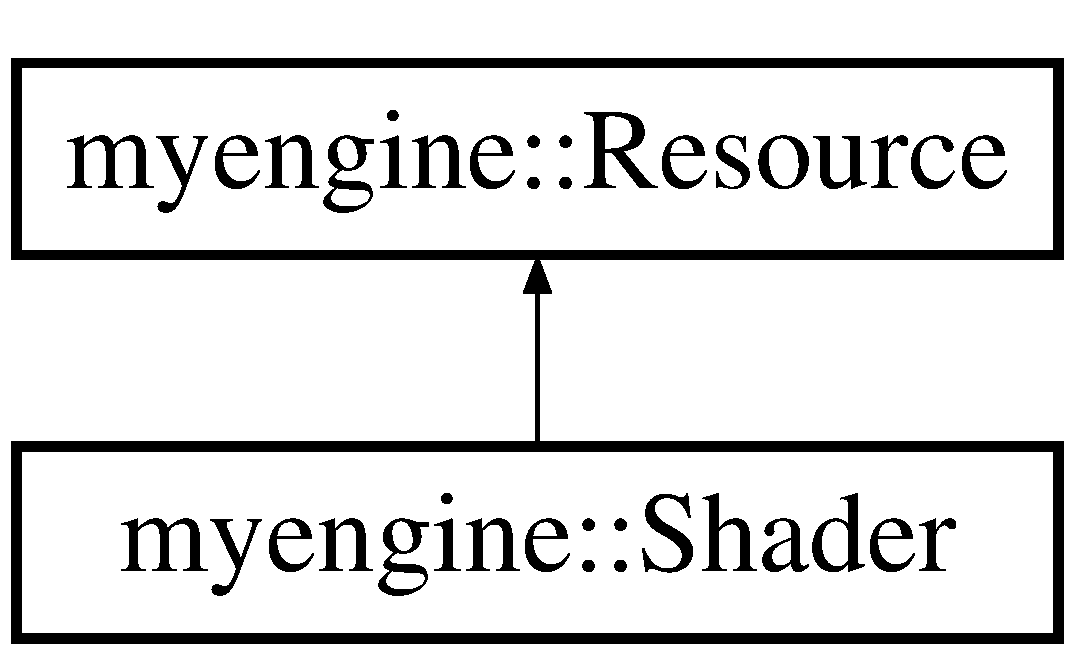
\includegraphics[height=2.000000cm]{classmyengine_1_1_shader}
\end{center}
\end{figure}
\subsection*{Public Member Functions}
\begin{DoxyCompactItemize}
\item 
\hyperlink{classmyengine_1_1_shader_aee2f3e6536000e55269b4f3a2f9c478f}{Shader} ()
\item 
\hyperlink{classmyengine_1_1_shader_a857cbbb1aa3eb09212cadd9d5bd5edf9}{$\sim$\+Shader} ()
\item 
void \hyperlink{classmyengine_1_1_shader_ac73d2e97c8afd63cc0b826f596dd330e}{Set\+Uniform} (G\+Lchar $\ast$\+\_\+name, float \+\_\+value, bool \+\_\+unset\+Program=false)
\item 
void \hyperlink{classmyengine_1_1_shader_a8f90d7986843c6e462f51b574fb2494a}{Set\+Uniform} (G\+Lchar $\ast$\+\_\+name, std\+::weak\+\_\+ptr$<$ \hyperlink{classmyengine_1_1_texture}{Texture} $>$ \+\_\+texture, bool \+\_\+unset\+Program=false)
\item 
void \hyperlink{classmyengine_1_1_shader_a3a1a27a7aaa38dad35d2505e4b99380f}{Set\+Uniform} (G\+Lchar $\ast$\+\_\+name, glm\+::mat4 \+\_\+value, bool \+\_\+unset\+Program=false, bool \+\_\+transpose=false)
\item 
void \hyperlink{classmyengine_1_1_shader_a63e19986143ad7857d270e22ea0a4ff0}{Set\+Uniform} (G\+Lchar $\ast$\+\_\+name, glm\+::vec3 \+\_\+value, bool \+\_\+unset\+Program=false)
\item 
void \hyperlink{classmyengine_1_1_shader_a9753467c609016a7c1c7a1156da2533f}{set\+ID} (G\+Luint \+\_\+new\+ID)
\item 
G\+Luint \hyperlink{classmyengine_1_1_shader_a2849648cdf31caa5c0ba50a639091387}{get\+ID} ()
\end{DoxyCompactItemize}
\subsection*{Static Public Member Functions}
\begin{DoxyCompactItemize}
\item 
static std\+::shared\+\_\+ptr$<$ \hyperlink{classmyengine_1_1_shader}{Shader} $>$ \hyperlink{classmyengine_1_1_shader_a0b65f89c7c9813f76c17a3e4a26b2ae5}{Create} (std\+::string \+\_\+frag\+Scr, std\+::string \+\_\+vert\+Scr, std\+::vector$<$ G\+Lchar $\ast$$>$ \+\_\+attributes, std\+::shared\+\_\+ptr$<$ \hyperlink{classmyengine_1_1_resources}{Resources} $>$ \+\_\+resources)
\end{DoxyCompactItemize}
\subsection*{Additional Inherited Members}


\subsection{Constructor \& Destructor Documentation}
\mbox{\Hypertarget{classmyengine_1_1_shader_aee2f3e6536000e55269b4f3a2f9c478f}\label{classmyengine_1_1_shader_aee2f3e6536000e55269b4f3a2f9c478f}} 
\index{myengine\+::\+Shader@{myengine\+::\+Shader}!Shader@{Shader}}
\index{Shader@{Shader}!myengine\+::\+Shader@{myengine\+::\+Shader}}
\subsubsection{\texorpdfstring{Shader()}{Shader()}}
{\footnotesize\ttfamily myengine\+::\+Shader\+::\+Shader (\begin{DoxyParamCaption}{ }\end{DoxyParamCaption})}

\mbox{\Hypertarget{classmyengine_1_1_shader_a857cbbb1aa3eb09212cadd9d5bd5edf9}\label{classmyengine_1_1_shader_a857cbbb1aa3eb09212cadd9d5bd5edf9}} 
\index{myengine\+::\+Shader@{myengine\+::\+Shader}!````~Shader@{$\sim$\+Shader}}
\index{````~Shader@{$\sim$\+Shader}!myengine\+::\+Shader@{myengine\+::\+Shader}}
\subsubsection{\texorpdfstring{$\sim$\+Shader()}{~Shader()}}
{\footnotesize\ttfamily myengine\+::\+Shader\+::$\sim$\+Shader (\begin{DoxyParamCaption}{ }\end{DoxyParamCaption})}



\subsection{Member Function Documentation}
\mbox{\Hypertarget{classmyengine_1_1_shader_a0b65f89c7c9813f76c17a3e4a26b2ae5}\label{classmyengine_1_1_shader_a0b65f89c7c9813f76c17a3e4a26b2ae5}} 
\index{myengine\+::\+Shader@{myengine\+::\+Shader}!Create@{Create}}
\index{Create@{Create}!myengine\+::\+Shader@{myengine\+::\+Shader}}
\subsubsection{\texorpdfstring{Create()}{Create()}}
{\footnotesize\ttfamily std\+::shared\+\_\+ptr$<$ \hyperlink{classmyengine_1_1_shader}{Shader} $>$ myengine\+::\+Shader\+::\+Create (\begin{DoxyParamCaption}\item[{std\+::string}]{\+\_\+frag\+Scr,  }\item[{std\+::string}]{\+\_\+vert\+Scr,  }\item[{std\+::vector$<$ G\+Lchar $\ast$$>$}]{\+\_\+attributes,  }\item[{std\+::shared\+\_\+ptr$<$ \hyperlink{classmyengine_1_1_resources}{Resources} $>$}]{\+\_\+resources }\end{DoxyParamCaption})\hspace{0.3cm}{\ttfamily [static]}}

\mbox{\Hypertarget{classmyengine_1_1_shader_a2849648cdf31caa5c0ba50a639091387}\label{classmyengine_1_1_shader_a2849648cdf31caa5c0ba50a639091387}} 
\index{myengine\+::\+Shader@{myengine\+::\+Shader}!get\+ID@{get\+ID}}
\index{get\+ID@{get\+ID}!myengine\+::\+Shader@{myengine\+::\+Shader}}
\subsubsection{\texorpdfstring{get\+I\+D()}{getID()}}
{\footnotesize\ttfamily G\+Luint myengine\+::\+Shader\+::get\+ID (\begin{DoxyParamCaption}{ }\end{DoxyParamCaption})}

\mbox{\Hypertarget{classmyengine_1_1_shader_a9753467c609016a7c1c7a1156da2533f}\label{classmyengine_1_1_shader_a9753467c609016a7c1c7a1156da2533f}} 
\index{myengine\+::\+Shader@{myengine\+::\+Shader}!set\+ID@{set\+ID}}
\index{set\+ID@{set\+ID}!myengine\+::\+Shader@{myengine\+::\+Shader}}
\subsubsection{\texorpdfstring{set\+I\+D()}{setID()}}
{\footnotesize\ttfamily void myengine\+::\+Shader\+::set\+ID (\begin{DoxyParamCaption}\item[{G\+Luint}]{\+\_\+new\+ID }\end{DoxyParamCaption})}

\mbox{\Hypertarget{classmyengine_1_1_shader_ac73d2e97c8afd63cc0b826f596dd330e}\label{classmyengine_1_1_shader_ac73d2e97c8afd63cc0b826f596dd330e}} 
\index{myengine\+::\+Shader@{myengine\+::\+Shader}!Set\+Uniform@{Set\+Uniform}}
\index{Set\+Uniform@{Set\+Uniform}!myengine\+::\+Shader@{myengine\+::\+Shader}}
\subsubsection{\texorpdfstring{Set\+Uniform()}{SetUniform()}\hspace{0.1cm}{\footnotesize\ttfamily [1/4]}}
{\footnotesize\ttfamily void myengine\+::\+Shader\+::\+Set\+Uniform (\begin{DoxyParamCaption}\item[{G\+Lchar $\ast$}]{\+\_\+name,  }\item[{float}]{\+\_\+value,  }\item[{bool}]{\+\_\+unset\+Program = {\ttfamily false} }\end{DoxyParamCaption})}

\mbox{\Hypertarget{classmyengine_1_1_shader_a8f90d7986843c6e462f51b574fb2494a}\label{classmyengine_1_1_shader_a8f90d7986843c6e462f51b574fb2494a}} 
\index{myengine\+::\+Shader@{myengine\+::\+Shader}!Set\+Uniform@{Set\+Uniform}}
\index{Set\+Uniform@{Set\+Uniform}!myengine\+::\+Shader@{myengine\+::\+Shader}}
\subsubsection{\texorpdfstring{Set\+Uniform()}{SetUniform()}\hspace{0.1cm}{\footnotesize\ttfamily [2/4]}}
{\footnotesize\ttfamily void myengine\+::\+Shader\+::\+Set\+Uniform (\begin{DoxyParamCaption}\item[{G\+Lchar $\ast$}]{\+\_\+name,  }\item[{std\+::weak\+\_\+ptr$<$ \hyperlink{classmyengine_1_1_texture}{Texture} $>$}]{\+\_\+texture,  }\item[{bool}]{\+\_\+unset\+Program = {\ttfamily false} }\end{DoxyParamCaption})}

\mbox{\Hypertarget{classmyengine_1_1_shader_a3a1a27a7aaa38dad35d2505e4b99380f}\label{classmyengine_1_1_shader_a3a1a27a7aaa38dad35d2505e4b99380f}} 
\index{myengine\+::\+Shader@{myengine\+::\+Shader}!Set\+Uniform@{Set\+Uniform}}
\index{Set\+Uniform@{Set\+Uniform}!myengine\+::\+Shader@{myengine\+::\+Shader}}
\subsubsection{\texorpdfstring{Set\+Uniform()}{SetUniform()}\hspace{0.1cm}{\footnotesize\ttfamily [3/4]}}
{\footnotesize\ttfamily void myengine\+::\+Shader\+::\+Set\+Uniform (\begin{DoxyParamCaption}\item[{G\+Lchar $\ast$}]{\+\_\+name,  }\item[{glm\+::mat4}]{\+\_\+value,  }\item[{bool}]{\+\_\+unset\+Program = {\ttfamily false},  }\item[{bool}]{\+\_\+transpose = {\ttfamily false} }\end{DoxyParamCaption})}

\mbox{\Hypertarget{classmyengine_1_1_shader_a63e19986143ad7857d270e22ea0a4ff0}\label{classmyengine_1_1_shader_a63e19986143ad7857d270e22ea0a4ff0}} 
\index{myengine\+::\+Shader@{myengine\+::\+Shader}!Set\+Uniform@{Set\+Uniform}}
\index{Set\+Uniform@{Set\+Uniform}!myengine\+::\+Shader@{myengine\+::\+Shader}}
\subsubsection{\texorpdfstring{Set\+Uniform()}{SetUniform()}\hspace{0.1cm}{\footnotesize\ttfamily [4/4]}}
{\footnotesize\ttfamily void myengine\+::\+Shader\+::\+Set\+Uniform (\begin{DoxyParamCaption}\item[{G\+Lchar $\ast$}]{\+\_\+name,  }\item[{glm\+::vec3}]{\+\_\+value,  }\item[{bool}]{\+\_\+unset\+Program = {\ttfamily false} }\end{DoxyParamCaption})}



The documentation for this class was generated from the following files\+:\begin{DoxyCompactItemize}
\item 
src/myengine/\hyperlink{_shader_8h}{Shader.\+h}\item 
src/myengine/\hyperlink{_shader_8cpp}{Shader.\+cpp}\end{DoxyCompactItemize}

\hypertarget{classmyengine_1_1_texture}{}\section{myengine\+:\+:Texture Class Reference}
\label{classmyengine_1_1_texture}\index{myengine\+::\+Texture@{myengine\+::\+Texture}}


{\ttfamily \#include $<$Texture.\+h$>$}

Inheritance diagram for myengine\+:\+:Texture\+:\begin{figure}[H]
\begin{center}
\leavevmode
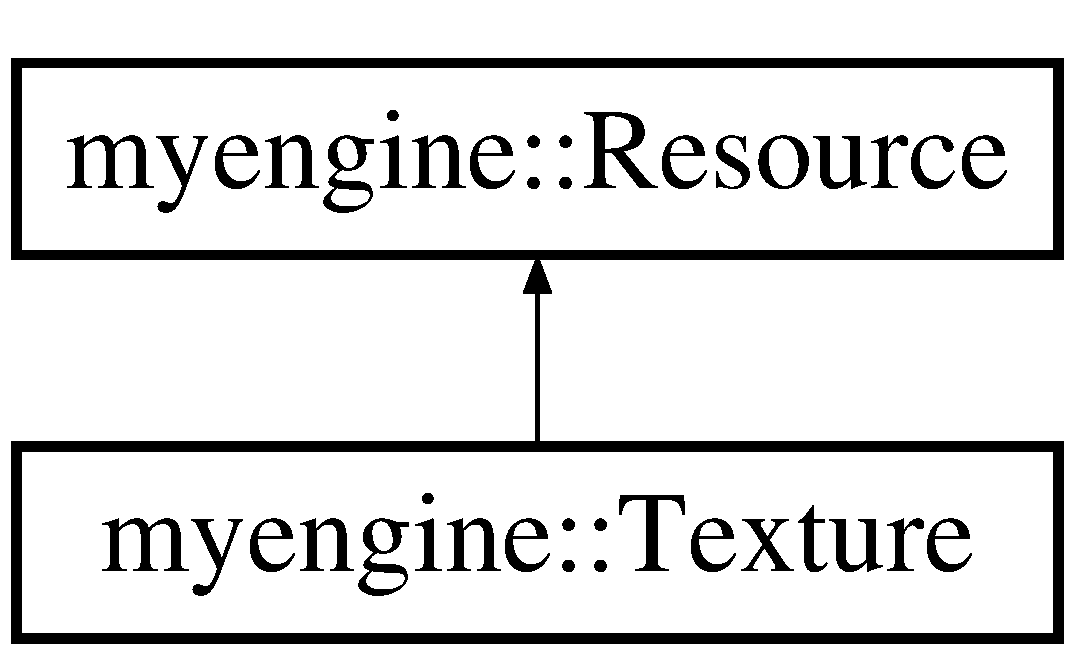
\includegraphics[height=2.000000cm]{classmyengine_1_1_texture}
\end{center}
\end{figure}
\subsection*{Public Member Functions}
\begin{DoxyCompactItemize}
\item 
void \hyperlink{classmyengine_1_1_texture_af178f6cbc4278bcc884a5651025d3dd9}{Set\+Texture} (G\+Luint \+\_\+new\+ID)
\item 
G\+Luint \hyperlink{classmyengine_1_1_texture_a10d2ae38dd467e9504f40df51ffa3c05}{Get\+Texture} ()
\item 
int \hyperlink{classmyengine_1_1_texture_a0bd0dcd679577e615bebec083c2da604}{Get\+Texture\+Location} ()
\end{DoxyCompactItemize}
\subsection*{Static Public Member Functions}
\begin{DoxyCompactItemize}
\item 
static std\+::shared\+\_\+ptr$<$ \hyperlink{classmyengine_1_1_texture}{Texture} $>$ \hyperlink{classmyengine_1_1_texture_a9796bf3a45107868c9371b869ff5a4e1}{Create} (const char $\ast$\hyperlink{classmyengine_1_1_resource_af7057ebf099efbd80751c64d25c2c83d}{\+\_\+path}, std\+::shared\+\_\+ptr$<$ \hyperlink{classmyengine_1_1_resources}{Resources} $>$ \+\_\+resources, int \+\_\+texture\+Location)
\end{DoxyCompactItemize}
\subsection*{Additional Inherited Members}


\subsection{Member Function Documentation}
\mbox{\Hypertarget{classmyengine_1_1_texture_a9796bf3a45107868c9371b869ff5a4e1}\label{classmyengine_1_1_texture_a9796bf3a45107868c9371b869ff5a4e1}} 
\index{myengine\+::\+Texture@{myengine\+::\+Texture}!Create@{Create}}
\index{Create@{Create}!myengine\+::\+Texture@{myengine\+::\+Texture}}
\subsubsection{\texorpdfstring{Create()}{Create()}}
{\footnotesize\ttfamily std\+::shared\+\_\+ptr$<$ \hyperlink{classmyengine_1_1_texture}{Texture} $>$ myengine\+::\+Texture\+::\+Create (\begin{DoxyParamCaption}\item[{const char $\ast$}]{\+\_\+path,  }\item[{std\+::shared\+\_\+ptr$<$ \hyperlink{classmyengine_1_1_resources}{Resources} $>$}]{\+\_\+resources,  }\item[{int}]{\+\_\+texture\+Location }\end{DoxyParamCaption})\hspace{0.3cm}{\ttfamily [static]}}

\mbox{\Hypertarget{classmyengine_1_1_texture_a10d2ae38dd467e9504f40df51ffa3c05}\label{classmyengine_1_1_texture_a10d2ae38dd467e9504f40df51ffa3c05}} 
\index{myengine\+::\+Texture@{myengine\+::\+Texture}!Get\+Texture@{Get\+Texture}}
\index{Get\+Texture@{Get\+Texture}!myengine\+::\+Texture@{myengine\+::\+Texture}}
\subsubsection{\texorpdfstring{Get\+Texture()}{GetTexture()}}
{\footnotesize\ttfamily G\+Luint myengine\+::\+Texture\+::\+Get\+Texture (\begin{DoxyParamCaption}{ }\end{DoxyParamCaption})}

\mbox{\Hypertarget{classmyengine_1_1_texture_a0bd0dcd679577e615bebec083c2da604}\label{classmyengine_1_1_texture_a0bd0dcd679577e615bebec083c2da604}} 
\index{myengine\+::\+Texture@{myengine\+::\+Texture}!Get\+Texture\+Location@{Get\+Texture\+Location}}
\index{Get\+Texture\+Location@{Get\+Texture\+Location}!myengine\+::\+Texture@{myengine\+::\+Texture}}
\subsubsection{\texorpdfstring{Get\+Texture\+Location()}{GetTextureLocation()}}
{\footnotesize\ttfamily int myengine\+::\+Texture\+::\+Get\+Texture\+Location (\begin{DoxyParamCaption}{ }\end{DoxyParamCaption})}

\mbox{\Hypertarget{classmyengine_1_1_texture_af178f6cbc4278bcc884a5651025d3dd9}\label{classmyengine_1_1_texture_af178f6cbc4278bcc884a5651025d3dd9}} 
\index{myengine\+::\+Texture@{myengine\+::\+Texture}!Set\+Texture@{Set\+Texture}}
\index{Set\+Texture@{Set\+Texture}!myengine\+::\+Texture@{myengine\+::\+Texture}}
\subsubsection{\texorpdfstring{Set\+Texture()}{SetTexture()}}
{\footnotesize\ttfamily void myengine\+::\+Texture\+::\+Set\+Texture (\begin{DoxyParamCaption}\item[{G\+Luint}]{\+\_\+new\+ID }\end{DoxyParamCaption})}



The documentation for this class was generated from the following files\+:\begin{DoxyCompactItemize}
\item 
src/myengine/\hyperlink{_texture_8h}{Texture.\+h}\item 
src/myengine/\hyperlink{_texture_8cpp}{Texture.\+cpp}\end{DoxyCompactItemize}

\hypertarget{classmyengine_1_1_triangle_renderer}{}\section{myengine\+:\+:Triangle\+Renderer Class Reference}
\label{classmyengine_1_1_triangle_renderer}\index{myengine\+::\+Triangle\+Renderer@{myengine\+::\+Triangle\+Renderer}}


{\ttfamily \#include $<$Triangle\+Renderer.\+h$>$}

Inheritance diagram for myengine\+:\+:Triangle\+Renderer\+:\begin{figure}[H]
\begin{center}
\leavevmode
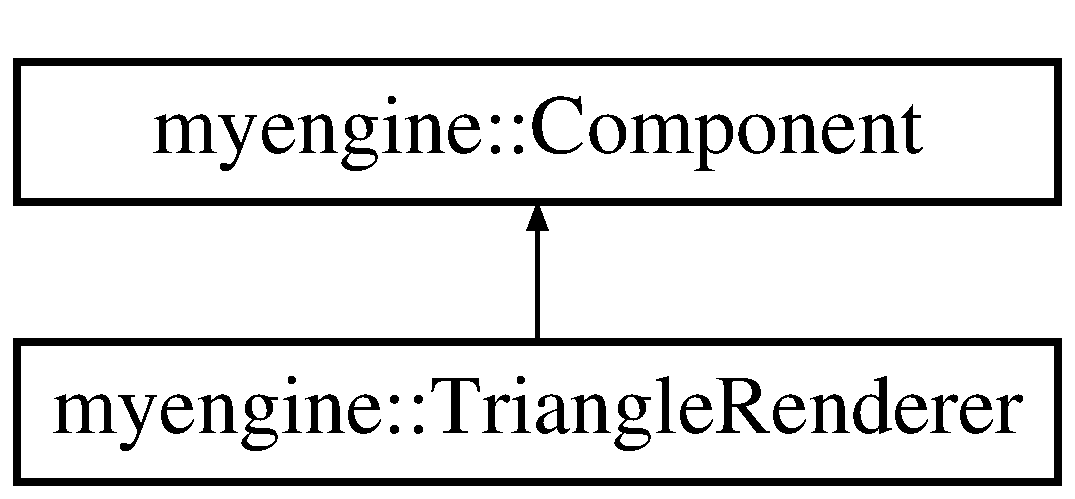
\includegraphics[height=2.000000cm]{classmyengine_1_1_triangle_renderer}
\end{center}
\end{figure}
\subsection*{Public Member Functions}
\begin{DoxyCompactItemize}
\item 
\hyperlink{classmyengine_1_1_triangle_renderer_a5b8c8b84f420ef262c0409a6fe5340b4}{Triangle\+Renderer} ()
\item 
\hyperlink{classmyengine_1_1_triangle_renderer_a5802b748911e8f3a4a4bbc2411c98ef7}{$\sim$\+Triangle\+Renderer} ()
\item 
void \hyperlink{classmyengine_1_1_triangle_renderer_aef2e04f1dd0419df1a60eb0cd95fd86c}{On\+Init} (std\+::weak\+\_\+ptr$<$ \hyperlink{classmyengine_1_1_entity}{Entity} $>$ \+\_\+parent) override
\item 
void \hyperlink{classmyengine_1_1_triangle_renderer_a74b0a056ed77e78a5061da2da6115bfd}{On\+Begin} () override
\item 
void \hyperlink{classmyengine_1_1_triangle_renderer_a6608a9c7954cff50e2575133dd6e5d88}{On\+Tick} () override
\item 
void \hyperlink{classmyengine_1_1_triangle_renderer_a266db93e50781c64232b16fe4f323bad}{On\+Display} () override
\item 
void \hyperlink{classmyengine_1_1_triangle_renderer_ae19ddcd41f6950a92744de0a17c43dbf}{Attach\+Shader\+Program} (std\+::shared\+\_\+ptr$<$ \hyperlink{classmyengine_1_1_shader}{Shader} $>$ \+\_\+new\+Shader\+Program)
\item 
std\+::shared\+\_\+ptr$<$ \hyperlink{classmyengine_1_1_shader}{Shader} $>$ \hyperlink{classmyengine_1_1_triangle_renderer_a4cc3d6924704e3cd2f2d9a499e1e93e7}{get\+Shader\+Program} ()
\item 
void \hyperlink{classmyengine_1_1_triangle_renderer_ab1c61a5a8ba4006e59e1838c69c54808}{Attach\+Texture} (std\+::shared\+\_\+ptr$<$ \hyperlink{classmyengine_1_1_texture}{Texture} $>$ \+\_\+new\+Texture)
\item 
std\+::shared\+\_\+ptr$<$ \hyperlink{classmyengine_1_1_texture}{Texture} $>$ \hyperlink{classmyengine_1_1_triangle_renderer_af5d1eae8138be9782577417eb8bd47ac}{get\+Texture} ()
\end{DoxyCompactItemize}
\subsection*{Additional Inherited Members}


\subsection{Constructor \& Destructor Documentation}
\mbox{\Hypertarget{classmyengine_1_1_triangle_renderer_a5b8c8b84f420ef262c0409a6fe5340b4}\label{classmyengine_1_1_triangle_renderer_a5b8c8b84f420ef262c0409a6fe5340b4}} 
\index{myengine\+::\+Triangle\+Renderer@{myengine\+::\+Triangle\+Renderer}!Triangle\+Renderer@{Triangle\+Renderer}}
\index{Triangle\+Renderer@{Triangle\+Renderer}!myengine\+::\+Triangle\+Renderer@{myengine\+::\+Triangle\+Renderer}}
\subsubsection{\texorpdfstring{Triangle\+Renderer()}{TriangleRenderer()}}
{\footnotesize\ttfamily myengine\+::\+Triangle\+Renderer\+::\+Triangle\+Renderer (\begin{DoxyParamCaption}{ }\end{DoxyParamCaption})}

\mbox{\Hypertarget{classmyengine_1_1_triangle_renderer_a5802b748911e8f3a4a4bbc2411c98ef7}\label{classmyengine_1_1_triangle_renderer_a5802b748911e8f3a4a4bbc2411c98ef7}} 
\index{myengine\+::\+Triangle\+Renderer@{myengine\+::\+Triangle\+Renderer}!````~Triangle\+Renderer@{$\sim$\+Triangle\+Renderer}}
\index{````~Triangle\+Renderer@{$\sim$\+Triangle\+Renderer}!myengine\+::\+Triangle\+Renderer@{myengine\+::\+Triangle\+Renderer}}
\subsubsection{\texorpdfstring{$\sim$\+Triangle\+Renderer()}{~TriangleRenderer()}}
{\footnotesize\ttfamily myengine\+::\+Triangle\+Renderer\+::$\sim$\+Triangle\+Renderer (\begin{DoxyParamCaption}{ }\end{DoxyParamCaption})}



\subsection{Member Function Documentation}
\mbox{\Hypertarget{classmyengine_1_1_triangle_renderer_ae19ddcd41f6950a92744de0a17c43dbf}\label{classmyengine_1_1_triangle_renderer_ae19ddcd41f6950a92744de0a17c43dbf}} 
\index{myengine\+::\+Triangle\+Renderer@{myengine\+::\+Triangle\+Renderer}!Attach\+Shader\+Program@{Attach\+Shader\+Program}}
\index{Attach\+Shader\+Program@{Attach\+Shader\+Program}!myengine\+::\+Triangle\+Renderer@{myengine\+::\+Triangle\+Renderer}}
\subsubsection{\texorpdfstring{Attach\+Shader\+Program()}{AttachShaderProgram()}}
{\footnotesize\ttfamily void myengine\+::\+Triangle\+Renderer\+::\+Attach\+Shader\+Program (\begin{DoxyParamCaption}\item[{std\+::shared\+\_\+ptr$<$ \hyperlink{classmyengine_1_1_shader}{Shader} $>$}]{\+\_\+new\+Shader\+Program }\end{DoxyParamCaption})}

\mbox{\Hypertarget{classmyengine_1_1_triangle_renderer_ab1c61a5a8ba4006e59e1838c69c54808}\label{classmyengine_1_1_triangle_renderer_ab1c61a5a8ba4006e59e1838c69c54808}} 
\index{myengine\+::\+Triangle\+Renderer@{myengine\+::\+Triangle\+Renderer}!Attach\+Texture@{Attach\+Texture}}
\index{Attach\+Texture@{Attach\+Texture}!myengine\+::\+Triangle\+Renderer@{myengine\+::\+Triangle\+Renderer}}
\subsubsection{\texorpdfstring{Attach\+Texture()}{AttachTexture()}}
{\footnotesize\ttfamily void myengine\+::\+Triangle\+Renderer\+::\+Attach\+Texture (\begin{DoxyParamCaption}\item[{std\+::shared\+\_\+ptr$<$ \hyperlink{classmyengine_1_1_texture}{Texture} $>$}]{\+\_\+new\+Texture }\end{DoxyParamCaption})}

\mbox{\Hypertarget{classmyengine_1_1_triangle_renderer_a4cc3d6924704e3cd2f2d9a499e1e93e7}\label{classmyengine_1_1_triangle_renderer_a4cc3d6924704e3cd2f2d9a499e1e93e7}} 
\index{myengine\+::\+Triangle\+Renderer@{myengine\+::\+Triangle\+Renderer}!get\+Shader\+Program@{get\+Shader\+Program}}
\index{get\+Shader\+Program@{get\+Shader\+Program}!myengine\+::\+Triangle\+Renderer@{myengine\+::\+Triangle\+Renderer}}
\subsubsection{\texorpdfstring{get\+Shader\+Program()}{getShaderProgram()}}
{\footnotesize\ttfamily std\+::shared\+\_\+ptr$<$ \hyperlink{classmyengine_1_1_shader}{Shader} $>$ myengine\+::\+Triangle\+Renderer\+::get\+Shader\+Program (\begin{DoxyParamCaption}{ }\end{DoxyParamCaption})}

\mbox{\Hypertarget{classmyengine_1_1_triangle_renderer_af5d1eae8138be9782577417eb8bd47ac}\label{classmyengine_1_1_triangle_renderer_af5d1eae8138be9782577417eb8bd47ac}} 
\index{myengine\+::\+Triangle\+Renderer@{myengine\+::\+Triangle\+Renderer}!get\+Texture@{get\+Texture}}
\index{get\+Texture@{get\+Texture}!myengine\+::\+Triangle\+Renderer@{myengine\+::\+Triangle\+Renderer}}
\subsubsection{\texorpdfstring{get\+Texture()}{getTexture()}}
{\footnotesize\ttfamily std\+::shared\+\_\+ptr$<$ \hyperlink{classmyengine_1_1_texture}{Texture} $>$ myengine\+::\+Triangle\+Renderer\+::get\+Texture (\begin{DoxyParamCaption}{ }\end{DoxyParamCaption})}

\mbox{\Hypertarget{classmyengine_1_1_triangle_renderer_a74b0a056ed77e78a5061da2da6115bfd}\label{classmyengine_1_1_triangle_renderer_a74b0a056ed77e78a5061da2da6115bfd}} 
\index{myengine\+::\+Triangle\+Renderer@{myengine\+::\+Triangle\+Renderer}!On\+Begin@{On\+Begin}}
\index{On\+Begin@{On\+Begin}!myengine\+::\+Triangle\+Renderer@{myengine\+::\+Triangle\+Renderer}}
\subsubsection{\texorpdfstring{On\+Begin()}{OnBegin()}}
{\footnotesize\ttfamily void myengine\+::\+Triangle\+Renderer\+::\+On\+Begin (\begin{DoxyParamCaption}{ }\end{DoxyParamCaption})\hspace{0.3cm}{\ttfamily [override]}, {\ttfamily [virtual]}}



Reimplemented from \hyperlink{classmyengine_1_1_component_ac852700a0c7227ca7229ae8c9ec4aa2d}{myengine\+::\+Component}.

\mbox{\Hypertarget{classmyengine_1_1_triangle_renderer_a266db93e50781c64232b16fe4f323bad}\label{classmyengine_1_1_triangle_renderer_a266db93e50781c64232b16fe4f323bad}} 
\index{myengine\+::\+Triangle\+Renderer@{myengine\+::\+Triangle\+Renderer}!On\+Display@{On\+Display}}
\index{On\+Display@{On\+Display}!myengine\+::\+Triangle\+Renderer@{myengine\+::\+Triangle\+Renderer}}
\subsubsection{\texorpdfstring{On\+Display()}{OnDisplay()}}
{\footnotesize\ttfamily void myengine\+::\+Triangle\+Renderer\+::\+On\+Display (\begin{DoxyParamCaption}{ }\end{DoxyParamCaption})\hspace{0.3cm}{\ttfamily [override]}, {\ttfamily [virtual]}}



Reimplemented from \hyperlink{classmyengine_1_1_component_ade43a7a8f4f8954b45ed05e1a8898eae}{myengine\+::\+Component}.

\mbox{\Hypertarget{classmyengine_1_1_triangle_renderer_aef2e04f1dd0419df1a60eb0cd95fd86c}\label{classmyengine_1_1_triangle_renderer_aef2e04f1dd0419df1a60eb0cd95fd86c}} 
\index{myengine\+::\+Triangle\+Renderer@{myengine\+::\+Triangle\+Renderer}!On\+Init@{On\+Init}}
\index{On\+Init@{On\+Init}!myengine\+::\+Triangle\+Renderer@{myengine\+::\+Triangle\+Renderer}}
\subsubsection{\texorpdfstring{On\+Init()}{OnInit()}}
{\footnotesize\ttfamily void myengine\+::\+Triangle\+Renderer\+::\+On\+Init (\begin{DoxyParamCaption}\item[{std\+::weak\+\_\+ptr$<$ \hyperlink{classmyengine_1_1_entity}{Entity} $>$}]{\+\_\+parent }\end{DoxyParamCaption})\hspace{0.3cm}{\ttfamily [override]}, {\ttfamily [virtual]}}



Reimplemented from \hyperlink{classmyengine_1_1_component_a66aeffd4cb32f438a4fc604e74e50057}{myengine\+::\+Component}.

\mbox{\Hypertarget{classmyengine_1_1_triangle_renderer_a6608a9c7954cff50e2575133dd6e5d88}\label{classmyengine_1_1_triangle_renderer_a6608a9c7954cff50e2575133dd6e5d88}} 
\index{myengine\+::\+Triangle\+Renderer@{myengine\+::\+Triangle\+Renderer}!On\+Tick@{On\+Tick}}
\index{On\+Tick@{On\+Tick}!myengine\+::\+Triangle\+Renderer@{myengine\+::\+Triangle\+Renderer}}
\subsubsection{\texorpdfstring{On\+Tick()}{OnTick()}}
{\footnotesize\ttfamily void myengine\+::\+Triangle\+Renderer\+::\+On\+Tick (\begin{DoxyParamCaption}{ }\end{DoxyParamCaption})\hspace{0.3cm}{\ttfamily [override]}, {\ttfamily [virtual]}}



Reimplemented from \hyperlink{classmyengine_1_1_component_ac84472ba368a622afa0e25c47757291a}{myengine\+::\+Component}.



The documentation for this class was generated from the following files\+:\begin{DoxyCompactItemize}
\item 
src/myengine/\hyperlink{_triangle_renderer_8h}{Triangle\+Renderer.\+h}\item 
src/myengine/\hyperlink{_triangle_renderer_8cpp}{Triangle\+Renderer.\+cpp}\end{DoxyCompactItemize}

\chapter{File Documentation}
\hypertarget{main_8cpp}{}\section{src/game/main.cpp File Reference}
\label{main_8cpp}\index{src/game/main.\+cpp@{src/game/main.\+cpp}}
{\ttfamily \#include $<$iostream$>$}\newline
{\ttfamily \#include $<$memory$>$}\newline
{\ttfamily \#include $<$myengine/\+My\+Engine.\+h$>$}\newline
{\ttfamily \#include $<$exception$>$}\newline
\subsection*{Functions}
\begin{DoxyCompactItemize}
\item 
void \hyperlink{main_8cpp_ac108aa5035d66c9a5e3c857b8e21df0b}{safe\+\_\+main} ()
\item 
int \hyperlink{main_8cpp_ae66f6b31b5ad750f1fe042a706a4e3d4}{main} ()
\end{DoxyCompactItemize}


\subsection{Function Documentation}
\mbox{\Hypertarget{main_8cpp_ae66f6b31b5ad750f1fe042a706a4e3d4}\label{main_8cpp_ae66f6b31b5ad750f1fe042a706a4e3d4}} 
\index{main.\+cpp@{main.\+cpp}!main@{main}}
\index{main@{main}!main.\+cpp@{main.\+cpp}}
\subsubsection{\texorpdfstring{main()}{main()}}
{\footnotesize\ttfamily int main (\begin{DoxyParamCaption}{ }\end{DoxyParamCaption})}

\mbox{\Hypertarget{main_8cpp_ac108aa5035d66c9a5e3c857b8e21df0b}\label{main_8cpp_ac108aa5035d66c9a5e3c857b8e21df0b}} 
\index{main.\+cpp@{main.\+cpp}!safe\+\_\+main@{safe\+\_\+main}}
\index{safe\+\_\+main@{safe\+\_\+main}!main.\+cpp@{main.\+cpp}}
\subsubsection{\texorpdfstring{safe\+\_\+main()}{safe\_main()}}
{\footnotesize\ttfamily void safe\+\_\+main (\begin{DoxyParamCaption}{ }\end{DoxyParamCaption})}


\hypertarget{_background_color_8cpp}{}\section{src/myengine/\+Background\+Color.cpp File Reference}
\label{_background_color_8cpp}\index{src/myengine/\+Background\+Color.\+cpp@{src/myengine/\+Background\+Color.\+cpp}}

\hypertarget{_background_color_8h}{}\section{src/myengine/\+Background\+Color.h File Reference}
\label{_background_color_8h}\index{src/myengine/\+Background\+Color.\+h@{src/myengine/\+Background\+Color.\+h}}
{\ttfamily \#include \char`\"{}glm.\+hpp\char`\"{}}\newline
{\ttfamily \#include \char`\"{}Component.\+h\char`\"{}}\newline
\subsection*{Classes}
\begin{DoxyCompactItemize}
\item 
class \hyperlink{classfrontier_1_1_back_ground_color}{frontier\+::\+Back\+Ground\+Color}
\end{DoxyCompactItemize}
\subsection*{Namespaces}
\begin{DoxyCompactItemize}
\item 
 \hyperlink{namespacefrontier}{frontier}
\end{DoxyCompactItemize}

\hypertarget{_component_8cpp}{}\section{src/myengine/\+Component.cpp File Reference}
\label{_component_8cpp}\index{src/myengine/\+Component.\+cpp@{src/myengine/\+Component.\+cpp}}
{\ttfamily \#include \char`\"{}Component.\+h\char`\"{}}\newline
{\ttfamily \#include \char`\"{}Entity.\+h\char`\"{}}\newline
{\ttfamily \#include \char`\"{}Core.\+h\char`\"{}}\newline
{\ttfamily \#include $<$iostream$>$}\newline
\subsection*{Namespaces}
\begin{DoxyCompactItemize}
\item 
 \hyperlink{namespacemyengine}{myengine}
\end{DoxyCompactItemize}

\hypertarget{_component_8h}{}\section{src/myengine/\+Component.h File Reference}
\label{_component_8h}\index{src/myengine/\+Component.\+h@{src/myengine/\+Component.\+h}}
{\ttfamily \#include $<$memory$>$}\newline
\subsection*{Classes}
\begin{DoxyCompactItemize}
\item 
class \hyperlink{classfrontier_1_1_component}{frontier\+::\+Component}
\end{DoxyCompactItemize}
\subsection*{Namespaces}
\begin{DoxyCompactItemize}
\item 
 \hyperlink{namespacefrontier}{frontier}
\end{DoxyCompactItemize}

\hypertarget{_core_8cpp}{}\section{src/myengine/\+Core.cpp File Reference}
\label{_core_8cpp}\index{src/myengine/\+Core.\+cpp@{src/myengine/\+Core.\+cpp}}
{\ttfamily \#include \char`\"{}Core.\+h\char`\"{}}\newline
{\ttfamily \#include \char`\"{}Entity.\+h\char`\"{}}\newline
{\ttfamily \#include \char`\"{}Environment.\+h\char`\"{}}\newline
{\ttfamily \#include \char`\"{}Resources.\+h\char`\"{}}\newline
{\ttfamily \#include \char`\"{}Camera.\+h\char`\"{}}\newline
{\ttfamily \#include \char`\"{}Input.\+h\char`\"{}}\newline
{\ttfamily \#include \char`\"{}Timer.\+h\char`\"{}}\newline
{\ttfamily \#include \char`\"{}Shader.\+h\char`\"{}}\newline
{\ttfamily \#include \char`\"{}Prefab.\+h\char`\"{}}\newline
{\ttfamily \#include \char`\"{}Pooler.\+h\char`\"{}}\newline
{\ttfamily \#include $<$iostream$>$}\newline
{\ttfamily \#include $<$G\+L/glew.\+h$>$}\newline
{\ttfamily \#include $<$map$>$}\newline
{\ttfamily \#include $<$exception$>$}\newline
\subsection*{Namespaces}
\begin{DoxyCompactItemize}
\item 
 \hyperlink{namespacefrontier}{frontier}
\end{DoxyCompactItemize}

\hypertarget{_core_8h}{}\section{src/myengine/\+Core.h File Reference}
\label{_core_8h}\index{src/myengine/\+Core.\+h@{src/myengine/\+Core.\+h}}
{\ttfamily \#include $<$memory$>$}\newline
{\ttfamily \#include $<$vector$>$}\newline
{\ttfamily \#include $<$S\+D\+L2/\+S\+D\+L.\+h$>$}\newline
{\ttfamily \#include \char`\"{}glm.\+hpp\char`\"{}}\newline
{\ttfamily \#include $<$string$>$}\newline
{\ttfamily \#include $<$A\+L/al.\+h$>$}\newline
{\ttfamily \#include $<$A\+L/alc.\+h$>$}\newline
\subsection*{Classes}
\begin{DoxyCompactItemize}
\item 
class \hyperlink{classfrontier_1_1_core}{frontier\+::\+Core}
\begin{DoxyCompactList}\small\item\em The main core of the engine. This is where all entities, prefabs and resources get created. \end{DoxyCompactList}\end{DoxyCompactItemize}
\subsection*{Namespaces}
\begin{DoxyCompactItemize}
\item 
 \hyperlink{namespacefrontier}{frontier}
\end{DoxyCompactItemize}

\hypertarget{_entity_8cpp}{}\section{src/myengine/\+Entity.cpp File Reference}
\label{_entity_8cpp}\index{src/myengine/\+Entity.\+cpp@{src/myengine/\+Entity.\+cpp}}
{\ttfamily \#include \char`\"{}Entity.\+h\char`\"{}}\newline
{\ttfamily \#include \char`\"{}Component.\+h\char`\"{}}\newline
{\ttfamily \#include \char`\"{}Transform.\+h\char`\"{}}\newline
{\ttfamily \#include \char`\"{}Prefab.\+h\char`\"{}}\newline
{\ttfamily \#include \char`\"{}Mesh\+Renderer.\+h\char`\"{}}\newline
{\ttfamily \#include \char`\"{}Collider.\+h\char`\"{}}\newline
{\ttfamily \#include \char`\"{}game/\+Asteroid\+Behavior.\+h\char`\"{}}\newline
{\ttfamily \#include \char`\"{}game/\+Projectile\+Behavior.\+h\char`\"{}}\newline
{\ttfamily \#include $<$iostream$>$}\newline
\subsection*{Namespaces}
\begin{DoxyCompactItemize}
\item 
 \hyperlink{namespacefrontier}{frontier}
\end{DoxyCompactItemize}

\hypertarget{_entity_8h}{}\section{src/myengine/\+Entity.h File Reference}
\label{_entity_8h}\index{src/myengine/\+Entity.\+h@{src/myengine/\+Entity.\+h}}
{\ttfamily \#include $<$vector$>$}\newline
{\ttfamily \#include $<$memory$>$}\newline
{\ttfamily \#include $<$type\+\_\+traits$>$}\newline
{\ttfamily \#include $<$typeinfo$>$}\newline
{\ttfamily \#include $<$iostream$>$}\newline
{\ttfamily \#include $<$assert.\+h$>$}\newline
{\ttfamily \#include \char`\"{}Component.\+h\char`\"{}}\newline
{\ttfamily \#include \char`\"{}glm.\+hpp\char`\"{}}\newline
\subsection*{Classes}
\begin{DoxyCompactItemize}
\item 
class \hyperlink{classfrontier_1_1_entity}{frontier\+::\+Entity}
\end{DoxyCompactItemize}
\subsection*{Namespaces}
\begin{DoxyCompactItemize}
\item 
 \hyperlink{namespacefrontier}{frontier}
\end{DoxyCompactItemize}

\hypertarget{_environment_8cpp}{}\section{src/myengine/\+Environment.cpp File Reference}
\label{_environment_8cpp}\index{src/myengine/\+Environment.\+cpp@{src/myengine/\+Environment.\+cpp}}
{\ttfamily \#include \char`\"{}Environment.\+h\char`\"{}}\newline
{\ttfamily \#include $<$iostream$>$}\newline
\subsection*{Namespaces}
\begin{DoxyCompactItemize}
\item 
 \hyperlink{namespacemyengine}{myengine}
\end{DoxyCompactItemize}

\hypertarget{_environment_8h}{}\section{src/myengine/\+Environment.h File Reference}
\label{_environment_8h}\index{src/myengine/\+Environment.\+h@{src/myengine/\+Environment.\+h}}
{\ttfamily \#include $<$S\+D\+L2/\+S\+D\+L.\+h$>$}\newline
{\ttfamily \#include $<$memory$>$}\newline
\subsection*{Classes}
\begin{DoxyCompactItemize}
\item 
class \hyperlink{classfrontier_1_1_environment}{frontier\+::\+Environment}
\end{DoxyCompactItemize}
\subsection*{Namespaces}
\begin{DoxyCompactItemize}
\item 
 \hyperlink{namespacefrontier}{frontier}
\end{DoxyCompactItemize}

\hypertarget{_input_8cpp}{}\section{src/myengine/\+Input.cpp File Reference}
\label{_input_8cpp}\index{src/myengine/\+Input.\+cpp@{src/myengine/\+Input.\+cpp}}

\hypertarget{_input_8h}{}\section{src/myengine/\+Input.h File Reference}
\label{_input_8h}\index{src/myengine/\+Input.\+h@{src/myengine/\+Input.\+h}}
{\ttfamily \#include $<$S\+D\+L2/\+S\+D\+L.\+h$>$}\newline
{\ttfamily \#include $<$S\+D\+L2/\+S\+D\+L\+\_\+keycode.\+h$>$}\newline
{\ttfamily \#include $<$memory$>$}\newline
{\ttfamily \#include $<$map$>$}\newline
{\ttfamily \#include \char`\"{}glm.\+hpp\char`\"{}}\newline
\subsection*{Classes}
\begin{DoxyCompactItemize}
\item 
class \hyperlink{classfrontier_1_1_input}{frontier\+::\+Input}
\end{DoxyCompactItemize}
\subsection*{Namespaces}
\begin{DoxyCompactItemize}
\item 
 \hyperlink{namespacefrontier}{frontier}
\end{DoxyCompactItemize}

\hypertarget{_mesh_8cpp}{}\section{src/myengine/\+Mesh.cpp File Reference}
\label{_mesh_8cpp}\index{src/myengine/\+Mesh.\+cpp@{src/myengine/\+Mesh.\+cpp}}

\hypertarget{_mesh_8h}{}\section{src/myengine/\+Mesh.h File Reference}
\label{_mesh_8h}\index{src/myengine/\+Mesh.\+h@{src/myengine/\+Mesh.\+h}}
{\ttfamily \#include \char`\"{}glm.\+hpp\char`\"{}}\newline
{\ttfamily \#include \char`\"{}Shader.\+h\char`\"{}}\newline
{\ttfamily \#include $<$string$>$}\newline
{\ttfamily \#include $<$vector$>$}\newline
{\ttfamily \#include $<$memory$>$}\newline
{\ttfamily \#include $<$G\+L/glew.\+h$>$}\newline
\subsection*{Classes}
\begin{DoxyCompactItemize}
\item 
class \hyperlink{classfrontier_1_1_mesh}{frontier\+::\+Mesh}
\begin{DoxyCompactList}\small\item\em Contains vertices, normals and texcoords loaded from an obj. \end{DoxyCompactList}\end{DoxyCompactItemize}
\subsection*{Namespaces}
\begin{DoxyCompactItemize}
\item 
 \hyperlink{namespacefrontier}{frontier}
\end{DoxyCompactItemize}

\hypertarget{_my_engine_8h}{}\section{src/myengine/\+My\+Engine.h File Reference}
\label{_my_engine_8h}\index{src/myengine/\+My\+Engine.\+h@{src/myengine/\+My\+Engine.\+h}}
{\ttfamily \#include \char`\"{}Component.\+h\char`\"{}}\newline
{\ttfamily \#include \char`\"{}Core.\+h\char`\"{}}\newline
{\ttfamily \#include \char`\"{}Entity.\+h\char`\"{}}\newline
{\ttfamily \#include \char`\"{}Environment.\+h\char`\"{}}\newline
{\ttfamily \#include \char`\"{}Input.\+h\char`\"{}}\newline
{\ttfamily \#include \char`\"{}Mesh.\+h\char`\"{}}\newline
{\ttfamily \#include \char`\"{}Resource.\+h\char`\"{}}\newline
{\ttfamily \#include \char`\"{}Shader.\+h\char`\"{}}\newline
{\ttfamily \#include \char`\"{}Texture.\+h\char`\"{}}\newline
{\ttfamily \#include \char`\"{}Resources.\+h\char`\"{}}\newline
{\ttfamily \#include \char`\"{}Camera.\+h\char`\"{}}\newline
{\ttfamily \#include \char`\"{}Transform.\+h\char`\"{}}\newline
{\ttfamily \#include \char`\"{}Mesh\+Renderer.\+h\char`\"{}}\newline
{\ttfamily \#include \char`\"{}Model.\+h\char`\"{}}\newline
{\ttfamily \#include \char`\"{}Sound.\+h\char`\"{}}\newline
{\ttfamily \#include \char`\"{}Audio\+Player.\+h\char`\"{}}\newline
{\ttfamily \#include \char`\"{}Skybox.\+h\char`\"{}}\newline
{\ttfamily \#include \char`\"{}Cubemap\+Texture.\+h\char`\"{}}\newline
{\ttfamily \#include \char`\"{}Collider.\+h\char`\"{}}\newline
{\ttfamily \#include \char`\"{}U\+I\+Image.\+h\char`\"{}}\newline
{\ttfamily \#include \char`\"{}U\+I\+Button.\+h\char`\"{}}\newline
{\ttfamily \#include \char`\"{}Prefab.\+h\char`\"{}}\newline
{\ttfamily \#include \char`\"{}Pooler.\+h\char`\"{}}\newline

\hypertarget{_resource_8cpp}{}\section{src/myengine/\+Resource.cpp File Reference}
\label{_resource_8cpp}\index{src/myengine/\+Resource.\+cpp@{src/myengine/\+Resource.\+cpp}}
{\ttfamily \#include \char`\"{}Resource.\+h\char`\"{}}\newline
{\ttfamily \#include $<$iostream$>$}\newline
\subsection*{Namespaces}
\begin{DoxyCompactItemize}
\item 
 \hyperlink{namespacefrontier}{frontier}
\end{DoxyCompactItemize}

\hypertarget{_resource_8h}{}\section{src/myengine/\+Resource.h File Reference}
\label{_resource_8h}\index{src/myengine/\+Resource.\+h@{src/myengine/\+Resource.\+h}}
{\ttfamily \#include $<$string$>$}\newline
{\ttfamily \#include $<$memory$>$}\newline
\subsection*{Classes}
\begin{DoxyCompactItemize}
\item 
class \hyperlink{classfrontier_1_1_resource}{frontier\+::\+Resource}
\begin{DoxyCompactList}\small\item\em Base class for a resource, all other resource types derive from this. \end{DoxyCompactList}\end{DoxyCompactItemize}
\subsection*{Namespaces}
\begin{DoxyCompactItemize}
\item 
 \hyperlink{namespacefrontier}{frontier}
\end{DoxyCompactItemize}

\hypertarget{_resources_8cpp}{}\section{src/myengine/\+Resources.cpp File Reference}
\label{_resources_8cpp}\index{src/myengine/\+Resources.\+cpp@{src/myengine/\+Resources.\+cpp}}
{\ttfamily \#include \char`\"{}Resources.\+h\char`\"{}}\newline
{\ttfamily \#include $<$iostream$>$}\newline
\subsection*{Namespaces}
\begin{DoxyCompactItemize}
\item 
 \hyperlink{namespacefrontier}{frontier}
\end{DoxyCompactItemize}

\hypertarget{_resources_8h}{}\section{src/myengine/\+Resources.h File Reference}
\label{_resources_8h}\index{src/myengine/\+Resources.\+h@{src/myengine/\+Resources.\+h}}
{\ttfamily \#include $<$list$>$}\newline
{\ttfamily \#include $<$memory$>$}\newline
{\ttfamily \#include \char`\"{}Resource.\+h\char`\"{}}\newline
\subsection*{Classes}
\begin{DoxyCompactItemize}
\item 
class \hyperlink{classmyengine_1_1_resources}{myengine\+::\+Resources}
\end{DoxyCompactItemize}
\subsection*{Namespaces}
\begin{DoxyCompactItemize}
\item 
 \hyperlink{namespacemyengine}{myengine}
\end{DoxyCompactItemize}

\hypertarget{_shader_8cpp}{}\section{src/myengine/\+Shader.cpp File Reference}
\label{_shader_8cpp}\index{src/myengine/\+Shader.\+cpp@{src/myengine/\+Shader.\+cpp}}
{\ttfamily \#include \char`\"{}Shader.\+h\char`\"{}}\newline
{\ttfamily \#include \char`\"{}Resources.\+h\char`\"{}}\newline
{\ttfamily \#include \char`\"{}Texture.\+h\char`\"{}}\newline
{\ttfamily \#include $<$fstream$>$}\newline
{\ttfamily \#include $<$sstream$>$}\newline
{\ttfamily \#include $<$iostream$>$}\newline
\subsection*{Namespaces}
\begin{DoxyCompactItemize}
\item 
 \hyperlink{namespacemyengine}{myengine}
\end{DoxyCompactItemize}

\hypertarget{_shader_8h}{}\section{src/myengine/\+Shader.h File Reference}
\label{_shader_8h}\index{src/myengine/\+Shader.\+h@{src/myengine/\+Shader.\+h}}
{\ttfamily \#include \char`\"{}Resource.\+h\char`\"{}}\newline
{\ttfamily \#include \char`\"{}glm.\+hpp\char`\"{}}\newline
{\ttfamily \#include $<$G\+L/glew.\+h$>$}\newline
{\ttfamily \#include $<$memory$>$}\newline
{\ttfamily \#include $<$vector$>$}\newline
\subsection*{Classes}
\begin{DoxyCompactItemize}
\item 
class \hyperlink{classfrontier_1_1_shader}{frontier\+::\+Shader}
\end{DoxyCompactItemize}
\subsection*{Namespaces}
\begin{DoxyCompactItemize}
\item 
 \hyperlink{namespacefrontier}{frontier}
\end{DoxyCompactItemize}

\hypertarget{_texture_8cpp}{}\section{src/myengine/\+Texture.cpp File Reference}
\label{_texture_8cpp}\index{src/myengine/\+Texture.\+cpp@{src/myengine/\+Texture.\+cpp}}
{\ttfamily \#include $<$iostream$>$}\newline
{\ttfamily \#include \char`\"{}Texture.\+h\char`\"{}}\newline
{\ttfamily \#include \char`\"{}Resources.\+h\char`\"{}}\newline
{\ttfamily \#include \char`\"{}stb\+\_\+image.\+h\char`\"{}}\newline
\subsection*{Namespaces}
\begin{DoxyCompactItemize}
\item 
 \hyperlink{namespacemyengine}{myengine}
\end{DoxyCompactItemize}
\subsection*{Macros}
\begin{DoxyCompactItemize}
\item 
\#define \hyperlink{_texture_8cpp_a18372412ad2fc3ce1e3240b3cf0efe78}{S\+T\+B\+\_\+\+I\+M\+A\+G\+E\+\_\+\+I\+M\+P\+L\+E\+M\+E\+N\+T\+A\+T\+I\+ON}
\end{DoxyCompactItemize}


\subsection{Macro Definition Documentation}
\mbox{\Hypertarget{_texture_8cpp_a18372412ad2fc3ce1e3240b3cf0efe78}\label{_texture_8cpp_a18372412ad2fc3ce1e3240b3cf0efe78}} 
\index{Texture.\+cpp@{Texture.\+cpp}!S\+T\+B\+\_\+\+I\+M\+A\+G\+E\+\_\+\+I\+M\+P\+L\+E\+M\+E\+N\+T\+A\+T\+I\+ON@{S\+T\+B\+\_\+\+I\+M\+A\+G\+E\+\_\+\+I\+M\+P\+L\+E\+M\+E\+N\+T\+A\+T\+I\+ON}}
\index{S\+T\+B\+\_\+\+I\+M\+A\+G\+E\+\_\+\+I\+M\+P\+L\+E\+M\+E\+N\+T\+A\+T\+I\+ON@{S\+T\+B\+\_\+\+I\+M\+A\+G\+E\+\_\+\+I\+M\+P\+L\+E\+M\+E\+N\+T\+A\+T\+I\+ON}!Texture.\+cpp@{Texture.\+cpp}}
\subsubsection{\texorpdfstring{S\+T\+B\+\_\+\+I\+M\+A\+G\+E\+\_\+\+I\+M\+P\+L\+E\+M\+E\+N\+T\+A\+T\+I\+ON}{STB\_IMAGE\_IMPLEMENTATION}}
{\footnotesize\ttfamily \#define S\+T\+B\+\_\+\+I\+M\+A\+G\+E\+\_\+\+I\+M\+P\+L\+E\+M\+E\+N\+T\+A\+T\+I\+ON}


\hypertarget{_texture_8h}{}\section{src/myengine/\+Texture.h File Reference}
\label{_texture_8h}\index{src/myengine/\+Texture.\+h@{src/myengine/\+Texture.\+h}}
{\ttfamily \#include \char`\"{}Resource.\+h\char`\"{}}\newline
{\ttfamily \#include $<$memory$>$}\newline
{\ttfamily \#include $<$string$>$}\newline
{\ttfamily \#include $<$G\+L/glew.\+h$>$}\newline
\subsection*{Classes}
\begin{DoxyCompactItemize}
\item 
class \hyperlink{classfrontier_1_1_texture}{frontier\+::\+Texture}
\begin{DoxyCompactList}\small\item\em A container for an image, loaded externally. \end{DoxyCompactList}\end{DoxyCompactItemize}
\subsection*{Namespaces}
\begin{DoxyCompactItemize}
\item 
 \hyperlink{namespacefrontier}{frontier}
\end{DoxyCompactItemize}

\hypertarget{_triangle_renderer_8cpp}{}\section{src/myengine/\+Triangle\+Renderer.cpp File Reference}
\label{_triangle_renderer_8cpp}\index{src/myengine/\+Triangle\+Renderer.\+cpp@{src/myengine/\+Triangle\+Renderer.\+cpp}}
{\ttfamily \#include \char`\"{}Triangle\+Renderer.\+h\char`\"{}}\newline
{\ttfamily \#include \char`\"{}Shader.\+h\char`\"{}}\newline
{\ttfamily \#include \char`\"{}Texture.\+h\char`\"{}}\newline
{\ttfamily \#include \char`\"{}Entity.\+h\char`\"{}}\newline
{\ttfamily \#include \char`\"{}Transform.\+h\char`\"{}}\newline
{\ttfamily \#include \char`\"{}Core.\+h\char`\"{}}\newline
{\ttfamily \#include \char`\"{}Camera.\+h\char`\"{}}\newline
{\ttfamily \#include $<$iostream$>$}\newline
\subsection*{Namespaces}
\begin{DoxyCompactItemize}
\item 
 \hyperlink{namespacefrontier}{frontier}
\end{DoxyCompactItemize}

\hypertarget{_triangle_renderer_8h}{}\section{src/myengine/\+Triangle\+Renderer.h File Reference}
\label{_triangle_renderer_8h}\index{src/myengine/\+Triangle\+Renderer.\+h@{src/myengine/\+Triangle\+Renderer.\+h}}
{\ttfamily \#include $<$G\+L/glew.\+h$>$}\newline
{\ttfamily \#include $<$memory$>$}\newline
{\ttfamily \#include \char`\"{}Component.\+h\char`\"{}}\newline
{\ttfamily \#include \char`\"{}glm.\+hpp\char`\"{}}\newline
\subsection*{Classes}
\begin{DoxyCompactItemize}
\item 
class \hyperlink{classmyengine_1_1_triangle_renderer}{myengine\+::\+Triangle\+Renderer}
\end{DoxyCompactItemize}
\subsection*{Namespaces}
\begin{DoxyCompactItemize}
\item 
 \hyperlink{namespacemyengine}{myengine}
\end{DoxyCompactItemize}

%--- End generated contents ---

% Index
\backmatter
\newpage
\phantomsection
\clearemptydoublepage
\addcontentsline{toc}{chapter}{Index}
\printindex

\end{document}
